

\documentclass[12pt,times,onecolumn]{article}

%% Use the option review to obtain double line spacing
%% \documentclass[authoryear,preprint,review,12pt]{elsarticle}

%% Use the options 1p,twocolumn; 3p; 3p,twocolumn; 5p; or 5p,twocolumn
%% for a journal layout:
%% \documentclass[final,1p,times]{elsarticle}
%% \documentclass[final,1p,times,twocolumn]{elsarticle}
%% \documentclass[final,3p,times]{elsarticle}
%% \documentclass[final,3p,times,twocolumn]{elsarticle}
%% \documentclass[final,5p,times]{elsarticle}
%% \documentclass[final,5p,times,twocolumn]{elsarticle}

%% For including figures, graphicx.sty has been loaded in
%% elsarticle.cls. If you prefer to use the old commands
%% please give \usepackage{epsfig}

%% The amssymb package provides various useful mathematical symbols
\usepackage{amssymb}
\usepackage{amsmath}
\usepackage[hidelinks]{hyperref}
\usepackage{color}
\usepackage{multirow}
\usepackage{subcaption}
\usepackage{graphicx}
\usepackage[a4paper]{geometry}
\usepackage{pdfpages}
\usepackage{epstopdf}
\usepackage{glossaries}

%% The amsthm package provides extended theorem environments
%% \usepackage{amsthm}

%% The lineno packages adds line numbers. Start line numbering with
%% \begin{linenumbers}, end it with \end{linenumbers}. Or switch it on
%% for the whole article with \linenumbers.
%% \usepackage{lineno}


\newcommand{\ml}[1]{\textcolor{blue}{ Mathieu: #1}}
\newcommand{\fg}[1]{\textcolor{red}{ Felix: #1}}

\begin{document}
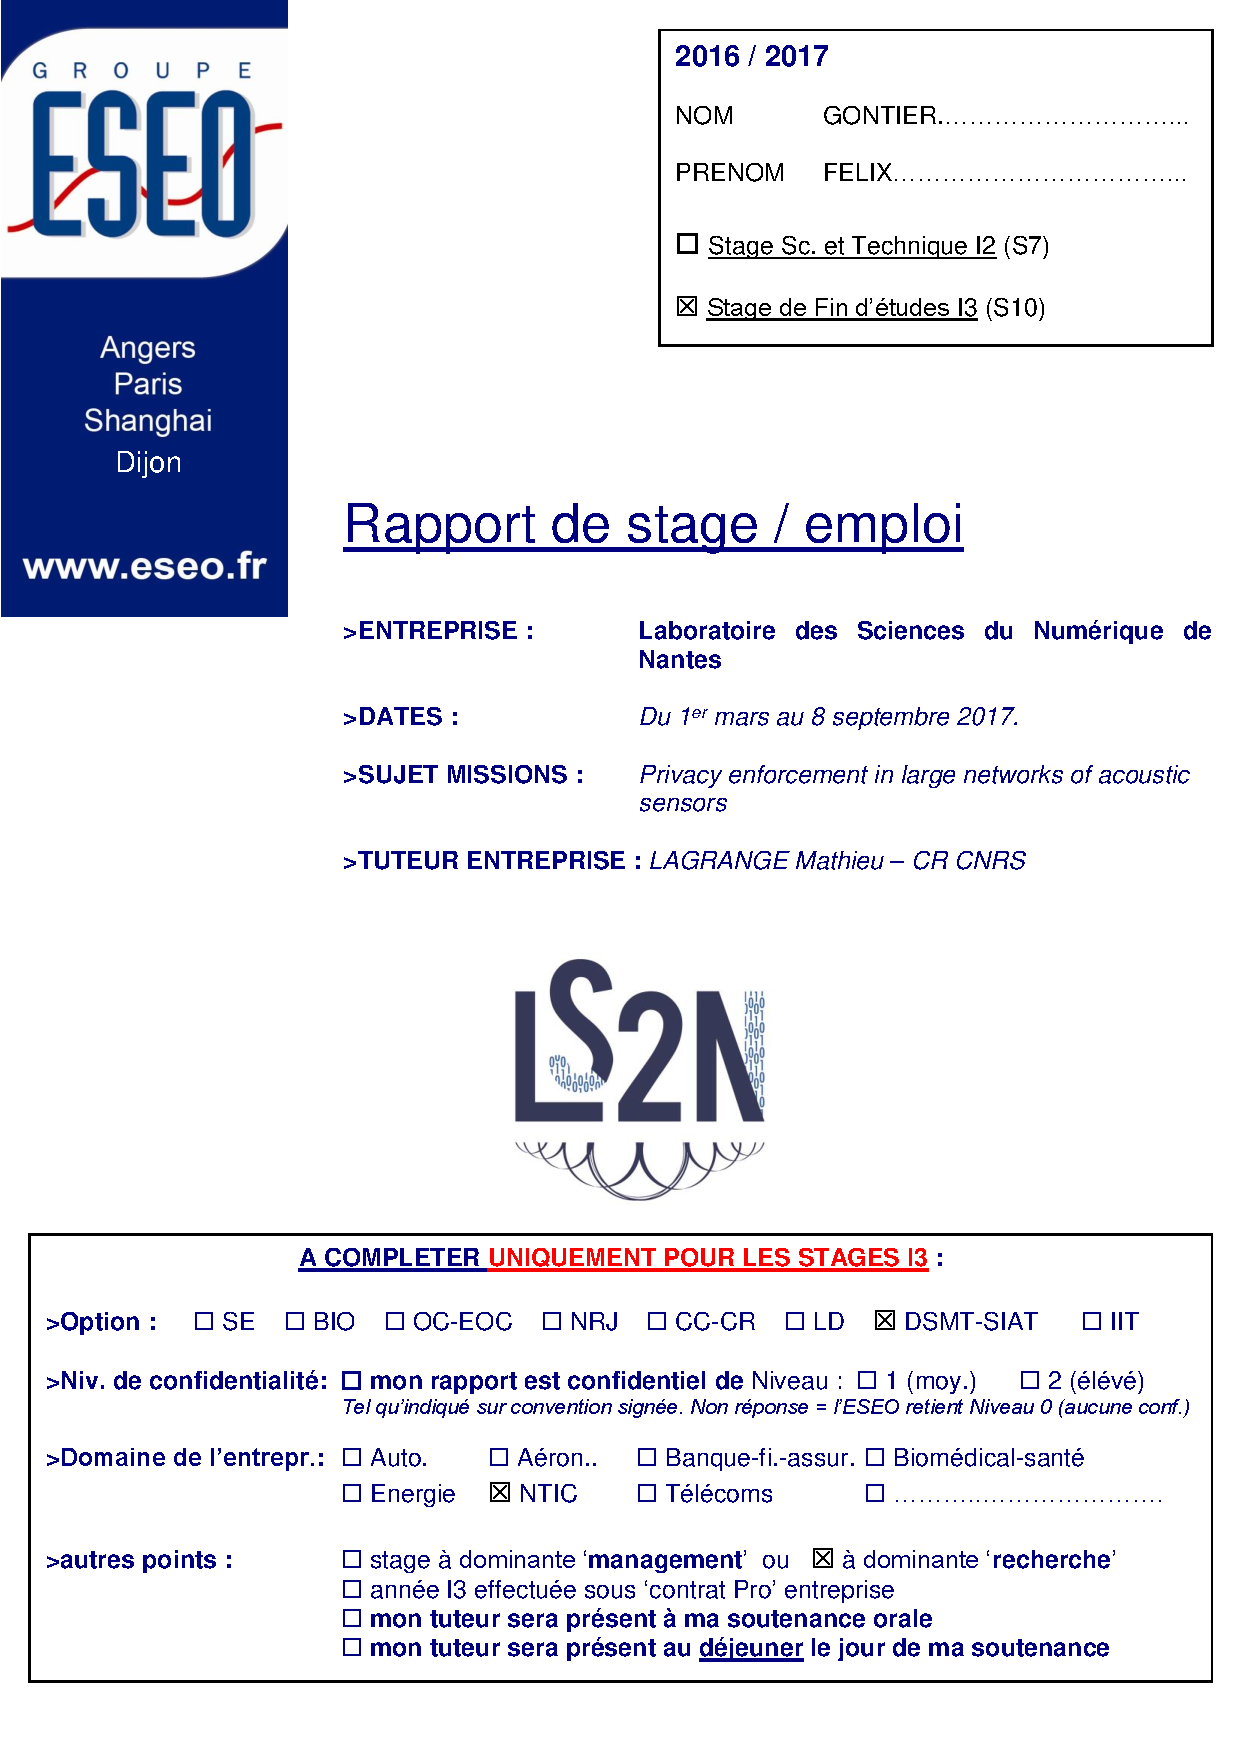
\includepdf[pages={1}]{cover.pdf}


\section*{Acknowledgements}

I am particularly grateful to Mathieu Lagrange who directed this internship. His close monitoring helped guide me throughout the many aspects of this experience.\\

I would like to thank Pierre Aumond at IFSTTAR for his broad contribution to the development of the coder, as well as to the written paper which he took the time to fully review several times. The fruitful discussions on fractional-octave band measurement error constituted an invaluable help.\\

I wish to thank Arnaud Can at IFSTTAR for his implication in the CENSE project and his interest in the present work. His insight and comments on the paper were particularly appreciated.\\

I express my gratitude to Jean-Rémy Gloaguen, PhD student at IFSTTAR/LS2N, for his sincere will to support my work with his extensive knowledge of acoustics.\\

I would like to thank Ludovic Charpentier, engineer at Wi6labs, for his patience regarding the embedded implementation of the proposed scheme.\\

I thank Catherine Lavandier of the Universit\'e de Cergy for her continued interest in my work, and along with Jean-François Petiot and Mathieu Lagrange for accepting to supervise my upcoming PhD thesis.

Finally, I would like to thank all the members of the Laboratoire des Sciences du Num\'erique de Nantes and of the CENSE project for their warm welcome into this internship and the research world in general.




\clearpage
\section*{Introduction}
\addcontentsline{toc}{section}{Introduction}
This report presents the masters internship proposed as part of the final year at ESEO with a two-fold objective. First, it was an opportunity to put to test both the technical knowledge and working skills learned during the five years of studies through an experience of long duration within a full company environment. Second, it aimed at finalizing the professional project developed at ESEO.\\

With respect to this last point, I had considered pursuing a PhD thesis in audio signal processing and machine-learning for a long time. The academic environment, the correlation with my expectations and the overall quality of ongoing works motivated my decision to apply at the Laboratoire des Sciences du Num\'erique de Nantes. I had the possibility to join the CENSE project and contribute to research on an ever-rising problem: noise management in large cities and more generally the understanding of urban soundscapes.\\

The internship's purpose was to enable continuous transmission of measured audio data through a city-scale sensor network. An audio coding scheme was necessary to satisfy several constraints linked to the size of the data, its information content for further processing concerns and the embedded hardware capabilities.\\

The first part of this report will provide contextual elements to the internship. A detailed explanation of the work contributing to the subject will be presented in the second part. Lastly, a third part will briefly reflect my view of the experience, as well as the many issues and opportunities faced during these past six months.


\clearpage
\section*{Internship summary}
\addcontentsline{toc}{section}{Internship summary}
\paragraph{Subject: Privacy enforcement in large networks of acoustic sensors\\}
This internship aimed at developing an audio processing and encoding scheme to enable continuous data recording in a large-scale embedded sensor network, as part of project CENSE. Among the technical constraints were low computational complexity, low output bitrate, and the ability to perform acoustic monitoring and sound event recognition tasks with the transmitted data. Additionally, decoded speech utterances were to be unintelligible to ensure the privacy of citizens. The involved themes are audio signal processing, acoustics, data coding and speech intelligibility.
\paragraph{Company\\}
Laboratoire des Sciences du Num\'erique de Nantes - \'Ecole Centrale de Nantes - Nantes, France.
\paragraph{Dates\\}
The internship took place between 1rst March 2017 and 8th September 2017, for a total duration of 28 weeks.
\paragraph{Team and contacts\\}
This internship was mostly composed of individual work. Regular exchanges were planned with my referent professor, M. Lagrange, to discuss about progress and planning concerns. I also worked with other members of the project from June to the end, including engineers at Wi6labs regarding an embedded implementation of the studied scheme and A. Can/P. Aumond at IFSTTAR about acoustic indicators and more generally the writing of the scientific paper.
\paragraph{Summarized planning\\}
\begin{itemize}
\item First two months: bibliographical research on acoustics and audio signal processing, study of datasets and classification methods, first version of the coder without computing acoustic indicators.
\item To early May: study of the coder's parameters effects on intelligibility indicators, classification tasks and bitrate.
\item Mid May to early June: computation of third-octave bands and paper writing beginning.
\item To the end of the internship: paper writing, intelligibility, measurement errors and sharing of this work with the project's teams.
\end{itemize}

\paragraph{Results\\}
The coder is completed, its parametrization as well as embedded implementation is being discussed with other members of the project. A study of the multiple involved factors is conducted with regard to the technical constraints. A scientific paper is also redacted and will be proposed for peer review and publication in the near future.


\clearpage
\tableofcontents
\clearpage
\listoffigures
\listoftables
\clearpage



\part{Context of the internship}
\section{LS2N: Laboratoire des Sciences du Num\'erique de Nantes}
The Laboratoire des Sciences du Num\'erique de Nantes (LS2N) which hosted this internship is a joint research unit (UMR6004) created in january 2017 as a result of the fusion of two research laboratories: the Institut de Recherche en Communication et Cybern\'etique de Nantes (IRCCyN) and the Laboratoire d'Informatique de Nantes Atlantique (LINA). It is under the supervision of the CNRS, the University of Nantes, the IMT, the \'Ecole Centrale de Nantes (ECN) and holds a partnership with the INRIA. The laboratory's activities are currently distributed over 5 sites in the city of Nantes, with the most important being located within the ECN's campus.\\

The LS2N's creation aimed at associating the local expertises on computer science and cybernetics. For this reason it contributes on a wide range of research areas:
\begin{itemize}
\item System Design and Operation (CCS) which focuses on embedded and industrial systems as well as general automation.
\item Robotics, Processes and Calculation (RPC) which studies the interactions of robots with their environment,
\item Data Science and Decision-making (SDD), with topics such as data modelling and classification,
\item Signals, Images, Ergonomics and Languages (SIEL) that takes interest in particular types of data related to human interactions and perception,
\item Software and Distributed Systems Science (SLS) which aims at solving software engineering challenges.
\end{itemize}
The domains of application are: industry of the future, management of energy and environmental impact, life sciences, vehicle and mobility, design, culture and digital society are all topics on which the LS2N has an expertise and influence.\\

The LS2N regroups 450 staff including researchers, engineers and PhD students. A total of 22 teams exist, each with its own members, research themes and projects. Lastly, the laboratory is involved in several academic programs in Nantes.

\section{The CENSE project}

The need to monitor and reduce noise pollution is nowadays a major concern, especially in urban environments where it is the most intense. To this aim, a few methods are commonly used to gather data relative to noise. First, noise maps are an efficient way to assess environmental boise pollution, and are regularly produced for large cities as required by the European Commission \cite{euc2002}. Current noise maps are mainly simulated with high-precision geographical data. They however rely on simplified sound source and propagation models that reduce the accuracy of the data. Additionnaly, the models do not consistently correlate with the human perception of a given sound event. Alternatively, observatories sample real sound signals. While these measurements are more accurate, they are very scarcely distributed in space and are thus insufficient to fully characterize soundscapes. Moreover, the existing observatories are often expensive to install and maintain.\\

\begin{figure}[htbp]
	\centering
		
\includegraphics[width=0.4\columnwidth]{figures/CENSE-logo.jpg}
	\caption{The project's logo.}
	\label{fig:cense_logo}
\end{figure}

The CENSE project, funded by the ANR (French national research funding agency), aims at proposing a viable solution to both noise maps construction and urban sound environment assessment. The main idea being developed is the deployment of a city-scale, dense low-cost sensor network to allow both measurement accuracy and geographical precision for noise maps. The recorded audio and physical indicators are to be used together with predicted data to combine these sources' advantages: accuracy and highly precise spatial information. The studied sensors are embedded low-power devices with wireless communication systems that are placed on public street lights. The city of Lorient was selected to develop this project.\\

The project is divided in six parts in its organization. Besides coordination, five interconnected units fragment the research objectives into development axes:
\begin{itemize}
\item The \textbf{Data and Modelling} intends to evaluate and improve uncertainties linked to simulated data by accessing exact measured values.
\item The \textbf{Measurement network} of which the present report is a part of aims at implementing a sensor network to match the above-mentionned needs and requirements.
\item The \textbf{Data assimilation} and network optimisation consists in associating the two previous units' outputs, respectively simulated and measured data, to best estimate noise levels in the considered environment.
\item The \textbf{Characterisation of sound environments} must use available data to better assess urban soundscape contents through indicators such as enhanced noise maps.
\end{itemize}
Finally, to promote accessibility and reproductibility of this work, another unit aspires to propose a software platform with all the project's data and a map application.\\

The project is coordinated by the Laboratoire d'Acoustique Environnementale (LAE) at IFSTTAR, although several other entities take part in its development. Their roles and actions are the following:
\begin{itemize}
\item The LAE and IFSTTAR also work on sensor placement and acoustical measurements processing,
\item The CNRS through the LS2N on data encoding with this internship and soundscape characterization,
\item Bouygues Energies and Services provide the energy and locations of embedded systems,
\item Wi6Labs implement the sensors and their hardware and software contents,
\item The Agence Nationale de la Recherche (ANR) funds the project.
\end{itemize}
Multiple disciplines and parties are involved with which this internship collaborates closely.

%\subsection{Sensor network}




\clearpage

\part{Detailed activities}
\setcounter{section}{0}
\section{Objectives}
This section describes the objectives pursued in the scope of this project.
\subsection{Audio coding in large scale sensor networks}
In the context of sensor network at a city scale, an important problem is to process the large amounts of audio signals that are continuously recorded. As the data is to be transmitted through wireless communication, the maximum bitrate allowed to a single sensor is severely insufficient for raw sound measurements. The scope of this work is to develop an audio coder so that all the data can be transferred to a remote server from the sensors.\\

The project primarily aims at processing data through two tasks: acoustic monitoring and audio event recognition. As will be developed later in this report, these two applications are different in the physical and mathematical concepts and quantities they involve. However, a common point is the use of relevant information extracted from audio signals instead of the raw data itself. This enables the use of transform functions to reduce bitrate. The proposed scheme must therefore employ a representation of the data in a way that efficiently makes both tasks possible.\\

Due to the coder being targeted to be implemented on embedded hardware other subsidiary constraints emerge, namely computational and memory costs. The target is a STM32L4 microcontroller with Cortex-M4 processor powered by solar energy. Operations are thus limited as well as data storage.\\

Finally, as sensors initially sample sound pressure, the privacy of citizen is an important concern. A study will be conducted on the intelligibility of encoded speech to ensure that both speakers and utterances content cannot be recognized.\\

Concerning implementation constraints during the project, they are as follow: the coder prototype is to be developed in Matlab, and evaluated using the expLanes \cite{explanes} framework. expLanes principle is to decompose projects into steps with a number of variable factors as inputs. A well defined project architecture is proposed which allows simple runs on different machines and operating systems. It also provides tools for results observation, report generation and execution parameters such as parallel processing. A GitHub repository must be maintained for both the project and a scientific paper presenting its characteristics.

\subsection{Acoustic monitoring}
The considered sensor network primarily aims at monitoring urban sound environment, that is, continuously assessing their content and impact on the population. In the literature, this is typically performed by measuring energetic acoustic indicators such as the equivalent sound pressure level $L_{eq}$ in dB SPL or its A-weighted equivalent $L_{Aeq}$ in dBA. However, while these indicators have proven to correlate well with perceptual evaluations for negative impact sound environments \cite{gozalo2015}, they are not sufficient to fully describe urban sound environments \cite{rychtarikova2013}. Many other variables can be derived to better account for previously implicit properties \cite{can2016} including percentile values or time dynamics. Studies have been conducted to select relevant subsets of descriptors in sound environment characterization \cite{can2015, brocolini2013, nilsson2007}. The mentionned $L_{eq}$ features are measured at periods of 0.125~ms or 1~s, respectively fast and slow as a convention.\\

Most measured or derived indicators describe the global urban soundscape and lack information on its composition. Sound sources recognition enables a more efficient understanding of soundscape properties. For instance, a bird song and traffic noise with the same energy can be perceived very differently. The analysis of sources within a sound environment is generally linked with spectral content \cite{ishiyama2000} and high temporal measurement resolutions. Other indicators can correlate with specific sound environment content \cite{aumond2017} but do not achieve the same performances as a source detection scheme in characterizing soundscapes.\\

A solution is the calculation of spectral energetic indicators such as the 31 third-octave bands within the human audition range 20~Hz - 20~kHz. Slow or fast third-octave bands measurement appears suitable for this work's purpose: in addition to being a relevant descriptor \cite{torija2013} for urban sound environment assessment, it allows for the computation of most cited indicators while representing reasonably small, fixed amounts of data to be transmitted. It additionnaly contains spectral information that can be used for source recognition tasks. However, as a tradeoff other representations such as Mel or Bark spectrograms, as well as psychoacoustical indicators cannot be precisely estimated.

\subsection{Audio event recognition}

As discussed in the previous section, the recognition of sources of interest is of importance to fully model the studied soundscapes. As far as the encoding scheme is concerned, it is thus primordial that the encoded data allows us to compute the above cited indicators but also to detect the different sound sources with state of the art methods.\\

The recognition of sources of interest from audio streams has been subject of extensive research in the past on speech \cite{anusuya2009}, music \cite{tzanetakis2002}, and lately more complex scenes in which the current work falls. Studied classification methods are diverse, ranging from time-dependant modeling with hidden markov models \cite{ntalampiras2014} to "bag-of-frames" approaches \cite{aucouturier2007, foggia2015}. Common architectures include learning-based classifiers such as support vector machines \cite{kumar2016}, Gaussian mixture models \cite{radhakrishnan2005} or neural networks \cite{salamon2017, piczak2015}. However, the selection of relevant features is still an open debate. The most used are certainly spectral \cite{khunarsal2013} or cepstral \cite{couvreur2004} representations of the signal. Among them, Mel spectrograms and their cepstral-domain derivation, the Mel-frequency cepstrum coefficients (MFCC), are the most recurrent. These representations effectively model the human cochlear response to sounds by grouping frequency components around critical bands in a logarithmic scale. While parameters are empirical and vary in the literature, a reference implementation includes 23.2~ms analysis and a 40 Mel bands resolution. The resulting representations are generally more precise in time and frequency than in acoustic monitoring applications because it is a primordial factor for classification whereas acoustic indicators must be computed more accurately.\\

They may also be exploited together with features computed in other domains to better model signal properties. For instance, \cite{cai2006} adds spectral features related to harmonicity and salient frequencies, and \cite{chu2009} uses a matching pursuit (MP) algorithm to deduce time-domain features. Another promising solution is feature engineering via unsupervised learning, which \cite{salamon2015-2} implements with a k-means clustering technique. Alternative data representations such as the scattering transform \cite{bauge2013} show good results in environmental sound classification tasks \cite{salamon2015}.\\
A more detailed review of used methods is available in \cite{chachada2013}.

\subsection{Intelligibility}
\label{sec:unintelligibility}
Intelligibility in decoded and reconstructed audio is also an important concern of this study. It is indeed important that the proposed scheme ensures a high level of recognition of acoustic events but, as the data is transmitted over the network and potentially stored, the level of intelligibility of the decoded stream should be as low as possible.\\

The use of an audio recording as an evidence is considered by the forensic phonetics \cite{baldwin1990forensic} domain. However, even with a good recording quality audio remains a weak biometrical indicator \cite{boe2000forensic}. Still, even if the identity of the speaker cannot be asserted, one can attempt to transcribe the spoken utterances. As such, it is important to demonstrate that the proposed encoding scheme effectively degrades intelligibility.\\

In order to ensure this property, several approaches can be considered. First, a speech versus non speech detector can be implemented on the sensor. If speech is detected, the data is not transmitted. This concept is however prone to failures of the detector and leads to the unavailability of data during speech periods. This is undesirable as it might compromise the computation of indicators which require time continuity.\\

Second, as the speech is mostly concentrated at frequencies ranging from 1 kHz to $~$4-5 kHz, a band-rejection filter located in this region could be considered in order to remove the formant information \cite{kent1992acoustic}. However, as some frequency bands are no longer available, the computation of standard acoustic indicators is no longer possible.\\

A third approach is to wisely choose the frame rate. Since a phoneme has a duration of about 100ms to 200ms \cite{kuwabara1996acoustic} \cite{rosen1992temporal} a frame rate lower than 4 Hz should dramatically reduce intelligibility.


\section{Coder scheme}

This section details the composition of the proposed coder scheme, as well as an introduction on the employed concepts and methods.

\subsection{Data representation}
\subsubsection{Short-Term Fourier Transform}
\label{stft}
To this day, the most commonly used tool for audio signal processing is the Fourier transform. This operation provides a mathematically simple, linear frequency analysis, with low computational complexity while remaining invertible. Despite the advent of more advanced methods such as the wavelet transform \cite{bentley1994}, most audio analysis, classification and synthesis schemes are thus still based on this transform. The two descriptors studied in this report can be obtained from the Fourier transform of a given input signal. As such, the discrete variant of this operation will be used as the first step of the coding scheme.\\

The Discrete Fourier Transform (DFT) of a signal $x[n]$ of arbitrary length $N>0$ is defined as
\begin{equation}
X[k] = \mathcal{F}\{x\} = \sum\limits_{n = 0}^{N-1} x[n]e^{-i2\pi k\frac{n}{N}}, k\in [0, N-1]
\end{equation}
where $k$ represents the frequency points. The first $N/2+1$ points correspond to the $[0, Fs/2]$ frequencies linearly spaced with a factor of $Fs/N$ for a given sampling rate $Fs$. Because the studied signals are real-valued, the remaining $N/2-1$ points are the complex conjugates of the first half of the representation. The \textit{resolution} of an analysis is defined as $Fs/N$ and provides information regarding the capacity to differenciate two close frequency components in the signal. In some cases the signal will be modified to increase the \textit{precision} of the analysis, \textit{i.e.} the interval between two adjacent frequency points. This can be obtained by zero-padding the signal, but is generally done for practical purposes as it does not increase resolution.

However, in practice the processed signals are rarely stationnary, meaning that the information content of the signal varies with time. The DFT does not account for such variations, and the analysis of a long signal using this transform is often inefficient. The Short-Term Fourier Transform (STFT) is introduced to solve this concern by applying a DFT on fixed-length portions of the signal. Its expression is
\begin{equation} \label{eq:2}
X[m, k] = \sum\limits_{n = 0}^{N-1} x[n]w[mR-n]e^{-j2\pi k\frac{n}{N}}
\end{equation}
where $w$ is a windowing function used to isolate analysis frames and $R$ represents the hop size in samples, that is the time interval between two consecutive frames. Unlike the DFT where an implicit unit rectangular window spanning over the whole signal is applied, the STFT explicitely requires a window function as a separate parameter.\\

When applying a Fourier transform on short signals, framing effects can appear due to the windowing function. The convolution theorem states that an element-wise multiplication in the time-domain is equivalent to a convolution in the Fourier space. For this reason, windowing effectively convolutes the pure frequency representation of the signal by the Fourier transform of the used function. This produces an effect known as spectral leakage. Figure~\ref{fig:fft_win} shows the Fourier transform of common windows. The rectangular window has a narrow main lobe, so that a FFT bin value is unaffected by its neighbours. However, its sidelobes gains are high (the first peak at -13~dB compared to the main lobe) and even far frequency components have an impact on a given bin. Conversely, the Hann window has a larger main lobe but the sidelobes rapidly decrease in amplitude. Finally, the gaussian window compromises between the two by displaying a better attenuation on the first sidelobes.

\begin{figure}[htbp]
	\centering
		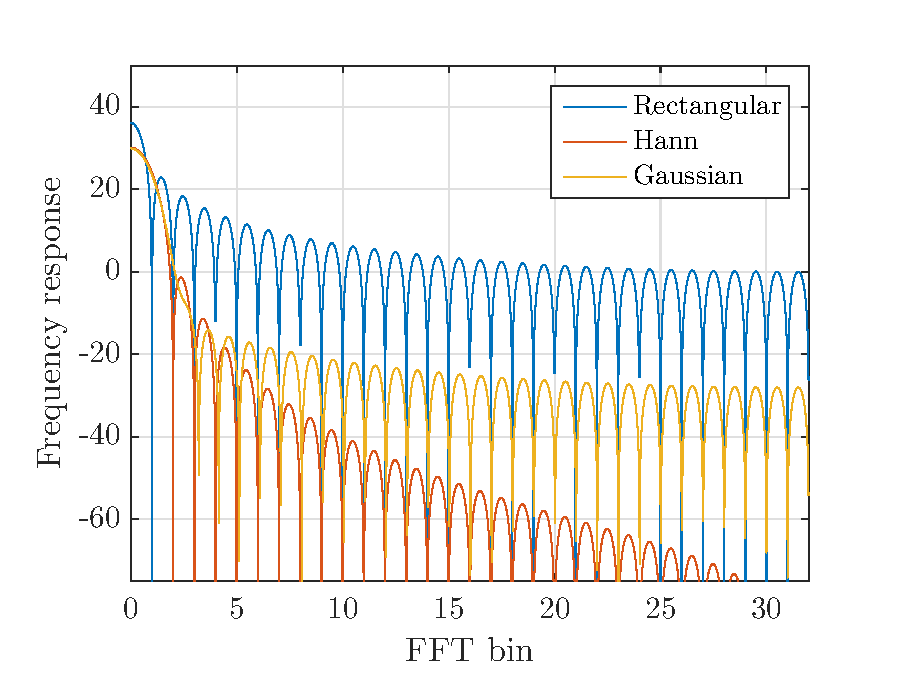
\includegraphics[width=0.5\columnwidth]{figures/fft_win.eps}
	\caption{Comparison of common windowing functions and their effect on the Fourier transform.}
	\label{fig:fft_win}
\end{figure}


Another property of the Fourier transform is the conservation of energy. Parseval's theorem states that the energy of the Fourier transform is equal to that of the time-domain signal up to a multiplicative constant:
\begin{equation}
\sum\limits_{n=0}^{N-1}|x[n]|^2 = \frac{1}{N}\sum\limits_{n=0}^{N-1}|X[k]|^2
\end{equation}
where $N$ is the length of the signal $x$. This is a necessary condition to the computation of third-octave bands for acoustic monitoring where the sound level is the main studied measurement.\\

In the coder application, the STFT of a continuously sampled signal is computed. As the studied descriptors depend only on the magnitude of the resulting spectrogram, the phase is discarded as well as the conjugate half. The choice of framing parameters as well as the windowing function will be discussed in the results section.

\subsubsection{Third-octave analysis}
The third-octave bands analysis consists in the application of bandpass filters with precise gains and cutoff frequencies. The measurement is then computed as the energy of each filtered result. The specifications for such filters are given by the ANSI S1.1-1986 \cite{citeulike:9580295} and IEC 61260-1:2014 \cite{iec-norm} standards. Additionally the IEC 61672-1:2013 \cite{iec-norm2} standard specifies band-wise tolerances determining the class of sound level meter developed: class 1 requires highly accurate measurements while class 2 has softer constraints. Globally the error should be low around the reference frequency of 1~kHz and is allowed to be larger at the edge bands, particularly at very low frequencies of 20-50~Hz.

\paragraph{Time-filtering\\\\}
The usual method \cite{davis1986} to perform fractional-octave analysis involves the design of time-domain FIR filters. The filter coefficients are computed for the highest desired octave and applied on progressively time-decimated versions of the input signal.\\

This operation is closely related to wavelet analysis in both design and complexity. However, its main limitation is given by the constraints of time-domain filter design such as ripples, slopes and causality conditions.

\paragraph{FFT-based filtering\\\\}
An alternative method is proposed in \cite{antoni2010} using the Fourier representation of the signal. The filters can then be defined as constant frequency weights, and the filtering operation as a matrix multiplication.\\

The cutoff frequencies are shared by adjacent bands. The frequency weights matrix is thus designed around the corresponding points $k_i$ as follows:
\begin{align}
G_i(k_i+p_i) &= sin\left(\frac{\pi}{2}\varphi_l(p_i)\right)\\
G_i(k_{i+1}+p_{i+1}) &= cos\left(\frac{\pi}{2}\varphi_l(p_{i+1})\right)\\
\varphi_l(p_i) &= sin\left(\frac{\pi}{2}\varphi_{l-1}(p_i)\right)\\
\varphi_0(p_i) &= \frac{1}{2}\left(\frac{p_i}{P_i}+1\right), p_i \in [-P_i, P_i]
\end{align}
where $P_i$ determines the frequency range where the weights are between 0 and 1 around each cutoff frequency, and the $l$ parameter controls the slope of the resulting filters. All other frequencies are assigned a weight of 1 between the increasing and decreasing part of a band, and 0 otherwise. Figure~\ref{fig:freq_filt} shows an example of bandpass filter computed with this process for different values of $l$ and compared to Couvreur's \cite{couvreur2004} time domain implementation.\\

\begin{figure}[htbp]
	\centering
		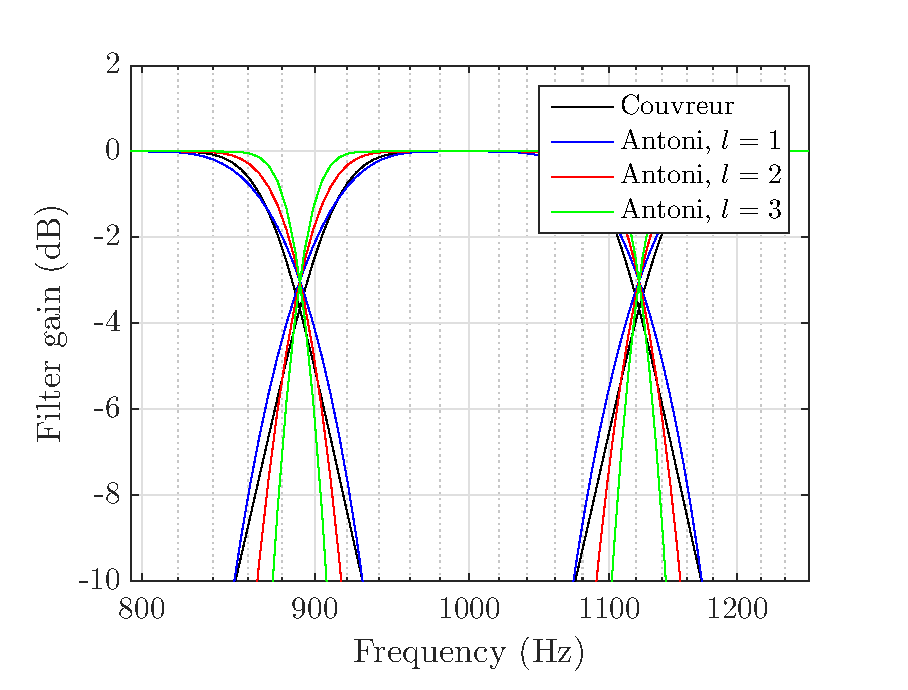
\includegraphics[width=0.5\columnwidth]{figures/tob_imp.eps}
	\caption{Comparison of Couvreur's and Antoni's implementations of third-octave filters. Frequency-weighting allows for arbitrary transfer functions and thus more accurate gains as standards impose.}
	\label{fig:freq_filt}
\end{figure}

\noindent This design ensures the following properties $\forall~l\geq 1$:
\begin{itemize}
\item The cutoff frequencies weights are fixed to -3dB
\item The energy of the signal is conserved over all bands, as the sum of the square of filter weights along bands equals 1 for all frequency points.
\end{itemize}
For $l = 2$ or $l = 3$, the filters are shown to be compliant with both the ANSI S1.1-1986 and IEC 61260-1:2014 standards. The calculation of third-octave bands is then:
\begin{equation}
X_{L_{eq}} = aG^{\circ2}|X|^{\circ2}
\end{equation}
where $a$ is a normalization factor applied for energy conservation, $X$ is given by equation~\ref{eq:2} and $\circ$ denotes an element-wise operation. The $log_{10}$ function can be applied to obtain third-octave bands in dB SPL.\\

Although this method allows for arbitrary filter design, it is limited by the framing effects inherent to the STFT, particularly visible in low frequencies. It is also apparently of lower computational complexity than time-filtering, and is thus preferred in the proposed coder scheme.

\subsection{Data encoding}
At this level in the coder process, the data is constituted of third-octave bands representations of the audio input signal. The data is accumulated over arbitrary durations to form texture frames to be transmitted. Depending on the time integration of 125~ms or 1~s and with 31 bands within the range of [20~Hz, 20~kHz], the representation is a matrix of size $8T\times 31$ or $T\times 31$ respectively for $T$ seconds texture frames. The data size can however be further reduced using source coding techniques.

\subsubsection{Notions on source and entropy coding}
Every signal follows a distribution which can be associated to a probability density function (PDF). Digital signals have limited possibility as to the different values they can take, depending on the type of data they are coded on. These values are referred to as symbols, and result in discrete probability distributions. The PDF then contain the precise probability of appearance of each symbol, and can be exploited to pair each symbol or group of symbols to a code of different size so that the output data size is minimized.\\

The Shannon entropy $H$ defines the least possible average code size per input symbol given a signal's distribution. It is expressed as:
\begin{equation}
H = \sum\limits_i p_ilog_n(p_i), i = 0,..,i
\end{equation}
where $p_i$ is the probability of appearance of the $i^{th}$ symbol and $n$ is the output representational base, usually 2 for binary outputs.

The entropy is therefore closely related to the PDF and the underlying information content of the data. It is minimum at $H = 0$ when the signal is deterministic, \textit{i.e.} when a single symbol with a probability of 1 appears. Conversely, it reaches a maximum for uniform distributions at $H = log_n(1/N)$ where N is the number of symbols. A low entropy is thus achieved for signals with few values appearing with high probabilities and a low range of possible symbols.\\

Entropy coding algorithms use symbol-probability pairs to approach entropy. Arithmetic \cite{witten1987} and Huffman \cite{huffman1952} coding are two examples, and the latter is studied in this work.

\subsubsection{Huffman coding}
The Huffman algorithm is as follow. For $n = 2$, symbols are sorted by probability of appearance, then a binary Huffman tree is constructed using the following principle: at each step, the two lowest probabilities are drawn from the list and associated in the tree. The sum of the two probabilities is then added back to the list. When the root of the tree attains the cumulated probability of 1, the symbols are assigned a variable-length code. Each layer away from the root adds a bit so that the highest probability symbol has a one-bit code while the rarest has the longest code. The resulting symbol-code pairs form a Huffman dictionnary which is then used to transcribe inputs. The size of separately encoded symbols using this method is optimal, that is the closest achievable to the data entropy. Huffman coding is a straightforward algorithm with few situational variants.

\subsubsection{Proposed algorithm}
To allow for minimal errors, the audio analysis step is computed using data types with sizes ranging from 16 to 64 bits per stored value. Directly applying a coding algorithm is thus inefficient due to large dictionnaries inducing high computational costs and output code dimensions. A quantization step is used to reduce the number of symbols to an acceptable amount of $2^q$ values for q-bit values.\\

However, an example of data distribution computed for environmental audio recordings is shown in Figure~\ref{fig:pdf}a. Third-octave measurements are concentrated in low values and linearly quantifying would result in most of the information being lost. The use of a logarithmic function solves this problem by "flattening" the PDF. Measurements are therefore expressed in dB, then quantized as visible in Figure~\ref{fig:pdf}b.\\

In order to enable better Huffman coding performances, the PDF must follow the principles discussed in section 2.2.1. As measurements are made continuously, third-octave bands values usually vary slowly. Especially when using overlap in the STFT, consecutive frames contain redundant information that can be eliminated. To this aim $\Delta$-compression is applied along the time dimension. It consists in subtracting each frame to the previous one to encode only variations in the signal. This has the desired effect of concentrating the probability of appearance around zero as shown in Figure~\ref{fig:pdf}c. $\Delta$-compression inherently doubles the maximum number of symbols: for a signal $x\in [0, N]$, the result is $x_\Delta \in [-N, N]$. This is easily outweighted by the effects on the PDF and the compression yields a significant efficiency increase of Huffman coding.\\

\begin{figure}[htbp]
	\centering
		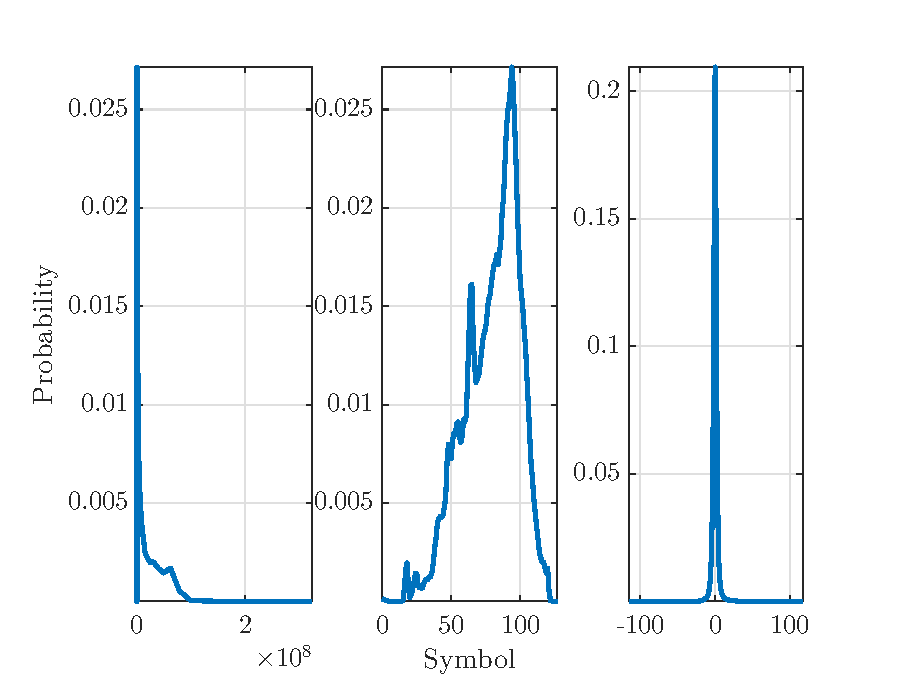
\includegraphics[width=0.7\textwidth]{figures/pdf.eps}
	\caption{Example of estimated probability density functions of the data throughout the encoding step. Unchanged output of the representation step (left), concentrated towards very low values. PDF "flattening" effect induced by logarithm application (middle). Here values are mapped to the range $[0, 2^7-1]$ and rounded to perform quantization. Output of the $\Delta$ compression (right) -, with desirable probabilities as the input to a Huffman algorithm.}
	\label{fig:pdf}
\end{figure}

One last choice regarding data encoding concerns the construction of the Huffman dictionnary. One solution is to generate a tree and dictionnary for each texture frame, which is then optimal but must be transmitted along with the code. Alternatively, a global dictionnary can be computed from large databases of environmental sounds. In that case, the coding process does not take into account the exact data distribution and must pair every possible symbol with a code. The added data of the first method and the sub-optimality of the second are found to compensate each other as they yield equivalent performances in this application. The computational complexity is found to be lower with dynamic dictionnary generation for a Matlab implementation, due to the number of symbols being generally between 2 and 5 time less than in the full dictionnary.

\subsection{Overview of the proposed scheme}
The coder scheme is summarized in Figure~\ref{fig:scheme}.

\begin{figure}[htbp]
	\centering
		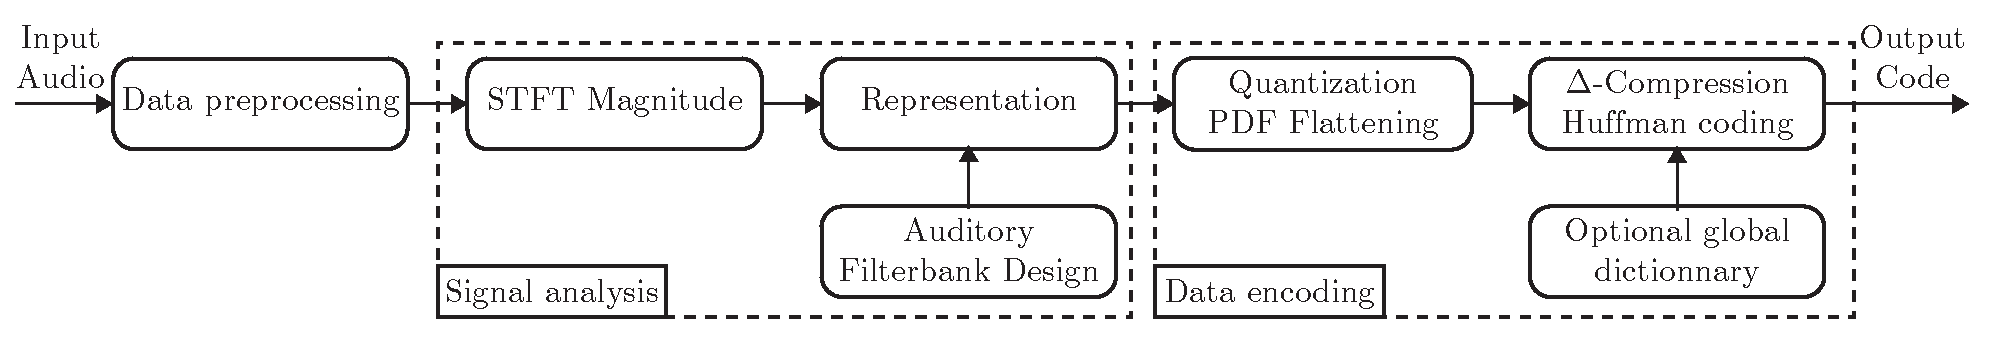
\includegraphics[width=1\textwidth]{figures/scheme.pdf}
	\caption{Overview of the coder processing scheme.}
	\label{fig:scheme}
\end{figure}
\section{Experimental validation setup}

\subsection{Datasets}
To evaluate the performances of the proposed coder, two datasets are used. The first consists of urban environmental audio recordings, and is used for measurement error, event recognition and bitrate concerns as its contents match the aim of the application. Furthermore, as unintelligibility is to be ensured in decoded and reconstructed audio extracts, a second dataset of clean speech recordings is studied.

\subsubsection{UrbanSound8k}
UrbanSound8k \cite{salamon2014} is a dataset of urban audio recordings proposed by the Sounds Of New-York City (SONYC) project researchers. It is composed of 8732 audio extracts with varying durations of less than 4~s, amounting to about 9 hours total. Each excerpt corresponds to one class among ten: \textit{street music}, \textit{child playing}, \textit{dog bark}, \textit{air conditionning}, \textit{drilling}, \textit{jackhammer}, \textit{car engine}, \textit{siren}, \textit{car horn}, \textit{gunshot}. The proportions are quite balanced with 1000 extracts per class except for the three last with about 900, 400 and 400 files respectively. The audio is provided at a sampling rate of 44.1~kHz in wave format which allows a degree of freedom as to the quality of the input data for testing purposes.\\

The UrbanSound8k dataset is a subset of a larger one, UrbanSound, made with the aim of providing a small but reliable resource for environmental audio applications such as classification. For this reason the data is distributed over 10 independant folds containing multiple examples of each class of sound, enabling cross-validation schemes. Several classification schemes and results are proposed for this dataset that can be used as a baseline, with techniques ranging from support vector machines and decision trees \cite{salamon2014} to deep learning \cite{salamon2017} with unsupervised feature learning \cite{salamon2015-2}.

\subsubsection{Speech recordings}
For intelligibility concerns, a small dataset of 23 clean speech recordings is used. This is to ensure the validity of the proposed test's results in the final implementation: if clean speech is made unintelligible, speech occurences in an environmental context where noise levels are important will be even harder to comprehend.\\

The dataset contains recordings of 9 french sentences enunciated by 6 different speakers, 3 of which are male and 3 female. This represent a total of 216 extracts of about 3 seconds each. The recordings were made in studio conditions and provided in 44.1~kHz stereo wave files.


\subsection{Measurement error}
The measurement error of third-octave bands is one of the main concerns of the coder validation, as this indicator is subject to strict tolerances. In the studied application, the error is two-fold: third-octave bands computation from raw audio is biased by framing the signal and the data encoding chain adds quantization error to the data.
\subsubsection{Analysis error}
To study the analysis error of third-octave bands, they can be compared to a trusted reference implementation. To this aim, third-octave bands measured in both "fast" computation with 125~ms windows and "slow" 1~s analysis mode are averaged over time to compute the acoustic indicator on extracts of several seconds. The chosen reference considers the Matlab \textit{ita\_ toolbox} implementation \cite{itatoolbox2017}. In both cases the sound dataset is the same and is composed of 2~s extracts. The experiment is run for white noise as well as urban environmental recordings. As the analysis frames are of short duration, poor frequency resolution and spectral leakage are expected, particularly in the lower frequencies bands. For this reason we evaluate the effect of the use of windowing functions on each band measurement error in order to mitigate this loss of precision. To provide relevant statistics, these quantities are estimated for about 4500 extracts obtained from the UrbanSound8k dataset \cite{salamon2014} and 4500 \textit{iid.} noise sequences.

\subsubsection{Additional encoding error}
The data encoding process is composed of lossless operations with the exception of quantization. The representation before this step is given in dB. Let us define $\varepsilon$ as the absolute error between the data $x$ and its quantized equivalent $x_q$, such as
\begin{equation}
\varepsilon = |x_q-x|
\end{equation}
The entire encoding process is defined by the desired Huffman dictionnary size $N_H$ which is linked to a word size $q$ with the relation
\begin{equation}
q = log_2(N_H)
\end{equation}
$q$ is obtained at the output of $\Delta$-compression. The values after quantization are thus coded on $q-1$ bits. $x_q$ is then given by:
\begin{equation}
x_q(n) = \frac{\Delta_x}{2^{q-1}-1}\textrm{round}\left(\frac{(2^{q-1}-1)x(n)}{\Delta_x}\right), x\in \left[0, \Delta_x\right]
\end{equation}
where $\Delta_x$ is the range of values taken by $x$. The error $\varepsilon$ can then be theoretically estimated by modelling the PDF of $x$ with a uniform distribution such as $x\sim \textit{U}\{0, \Delta_x\}$. While in reality $x$ will never be uniform, this approximation matches the aim of a decibel representation as discussed in section 2.2.3. $\varepsilon$ then also follows a uniform distribution $\varepsilon\sim U\{0, \frac{\Delta_x}{2\times (2^{q-1}-1)}\}$. Its mean $\mu_\varepsilon$ and standard deviation $\sigma_\varepsilon$ are:
\begin{equation} \label{eq:13}
\begin{cases}
	\mu_\epsilon = \frac{\Delta_x}{4\times (2^{q-1}-1)}\\
	\sigma_\epsilon = \frac{1}{12}\frac{\Delta_x}{2\times (2^{q-1}-1)}
\end{cases}
\end{equation}
In practice, the error is therefore assumed to be $\varepsilon = f(\Delta_x, \frac{1}{2^{q-1}-1})$ with the heterogeneity of the data's PDF inducing small variations to the equations in (12). Most mathematical operations such as base 10 logarithm and matrix multiplication can induce small additional rounding errors, especially on embedded implementations. Furthermore, the error should be the same across all third-octave bands as quantization operation is applied regardless of data dimensions.\\

The experimental evaluation consists in computing the absolute error for a set of word sizes $q$. The UrbanSound8k dataset is used to provide meaningful results both in audio data nature and number of examples.

\subsection{Output bitrate}

Another metric of the efficiency of the proposed scheme is the measurement of the output data bitrate. Similarly to classification, the parameters influencing the bitrate are the representation's time resolution and encoded word size $q$.

\subsection{Event recognition}

Descriptors based on third-octave bands analysis are relatively untested on classification tasks. In order to ensure that the proposed scheme allows the recognition of events using state of the art methods, it can be compared to the very similar and commonly used features derivated from mel bands analysis. Baseline performances \cite{salamon2014} are available for the UrbanSound8k dataset using Mel-Frequency Cepstrum Coefficients (MFCC), which are obtained by applying a Discrete Cosine Transform (DCT) to mel bands. The same operation is performed on third-octave bands to match the physical meaning of the MFCC descriptor.\\

The event recognition task performance is evaluated on four different models to ensure the validity of the results:
\begin{itemize}
\item a Support Vector Machine (SVM), which isolates data distributions of different classes by finding the maximum-margin separation between them. In this application, the C-SVM variant is used as a nonlinear classifier with a radial-basis function (RBF) kernel of variance $\sigma^2$. $C$ and $\sigma^2$ are found via grid search.
\item a Decision Tree (DT), that learns to take consecutive decisions based on the input features.
\item a Random Forest (RF) classifier, which is an ensemble method based on the decision tree. It uses the bagging concept of training several models and classifying by majority voting. The number of trees is here set to 500.
\item a k-Nearest Neighbors (KNN) classifier, which simply outputs the class of a test sample as that of the $k$ closest training examples. If N features characterize each data point, a N-dimensional mathematical distance is computed. In this evaluation the metric is the Euclidean distance and $k = 5$.
\end{itemize}

The features are computed from the 25 first mel or third-octave cepstrum coefficients, which as summarized along time with the mean, variance, skewness, kurtosis, minimum, maximum, median, derivative mean and variance, second order derivative mean and variance operators. The feature vector are thus comprised of 275 values. Each classifier is trained using 10-fold cross-validation which consists in training the models with 9 of the 10 folds and testing with the last, that for each of the 10 possible combinations.\\

For this process, the studied coder factors are the quantization word size $q$ and analysis frame duration. Mel spectrogram analysis is computed with the baseline 23~ms, 50\% overlap windows, then averaged over time to match the 125~ms or 1~s integration time used for third-octave bands measurements.

\subsection{Intelligibility assessment}

Encoding a raw audio recording should render it unintelligible at reconstruction. To guarantee this property the clean speech dataset presented in section 3.1.2 is passed through the encoding process, then decoded and recovered using methods detailed in Appendix~\ref{sigrec}. Intelligibility is then assessed using both objective and subjective indicators. Results will be shown for varying time resolutions during analysis only as the quantization was found to have very little impact on the perceived intelligibility.

\subsubsection{Objective indicators}

Intelligibility is known as an important factor in psychoacoustics and noisy environment studies. As a results, many objective indicators have been developed to model intelligibility based on either raw audio or spectral features. A review of these metrics is available in \cite{ma2009}. Various concepts and physical properties are exploited, although almost every method compares the noisy signal to a clean version. While several of the indicators are proved to correlate well with subjective estimations of intelligibility, results are only available for small degradations such as clipping and addition of white or colored noise. The studied signals experience much harsher conditions with band analysis and discarded phase spectrum. The accuracy of objective metrics is therefore not guaranteed and need to be compared to subjective evaluations.\\

Two indicators with good apparent results are computed: the Coherence-Speech Intelligibility Index (CSII) \cite{kates2005} and the Frequency-Weighted Segmental SNR (fwSNRseg) \cite{hu2008}.


\subsubsection{Perceptual test}
A perceptual intelligibility test is also conducted as both a reference for comparison with the objective indicators and an accurate evaluation to validate that the coder ensures privacy for the studied parameters.\\

The test is realised under the following conditions: a Matlab interface is displayed on a desktop computer. Each extract is played through \textit{Beyerdynamics DT 770} headphones in a random order. The output level is the same for all subjects. For each example, the participant is asked to type the words he understands and to rate the global intelligibility between 1 and 5. The Intelligibility Ratio (IR) \textit{i.e.} the percentage of correctly transcribed words constitutes the first subjective metric while the Average Intelligibility Score (AIS), that is the note scaled to 0 and 1, is a second indicator. 12 subjects of age ranging from 17 to 60 which reported normal hearing participated to the listening test.


\section{Results}
\subsection{Measurement error}
\paragraph{Analysis error\\\\}
The measurement error is computed for third-octave bands. Results are displayed in Figure~\ref{fig:error_m}. Only full-octave bands are shown for visibility. When computing the slow analysis, it is found that applying overlap attenuates the error. This is not observed for fast analysis where the error is similar or higher with the use of overlapping frames. As all experiments on noise show a mean error close to zero, the absolute error metric is preferred.\\

As can be expected when performing a short time analysis, high errors appear in low frequency bands where precision is poor. The slow analysis yields better estimations as it provides a globally better resolution and thus also reduces the impact of spectral leakage effects in this region. When considering white noise (left) the error is low on the whole spectrum. This effectiveness does not translate to environmental sounds analysis. A factor of this phenomenon is the sound level disparities absent in the first case but omnipresent in the second. In fact, spectral leakage induces a correlation between close frequency components as briefly explained in section~\ref{stft}. In lower frequencies, large differences between adjacent frequency bins can cause important errors on third-octave bands computations. This issue is however not specific to Fourier transform based schemes as it is also encountered with a time domain filtering approach.\\

To mitigate this phenomenon, the choice of the window function shall be studied further. For a fast analysis with no overlap, the rectangular window seems a reasonable choice at first with its energy conservation qualities. While it yields the lowest error in high frequency bands, its high spectral leakage effect makes it unprecise for lower frequency regions. Non-flat windows better account for this issue but require assuming that the signal is stationary in a given frame and are thus biased. For slow measurements, the rectangular window impact is less harmful to band analysis due to an increased frequency resolution.\\

\begin{figure*}[h!]
    \centering
    \begin{subfigure}[h]{0.45\textwidth}
        \centering
        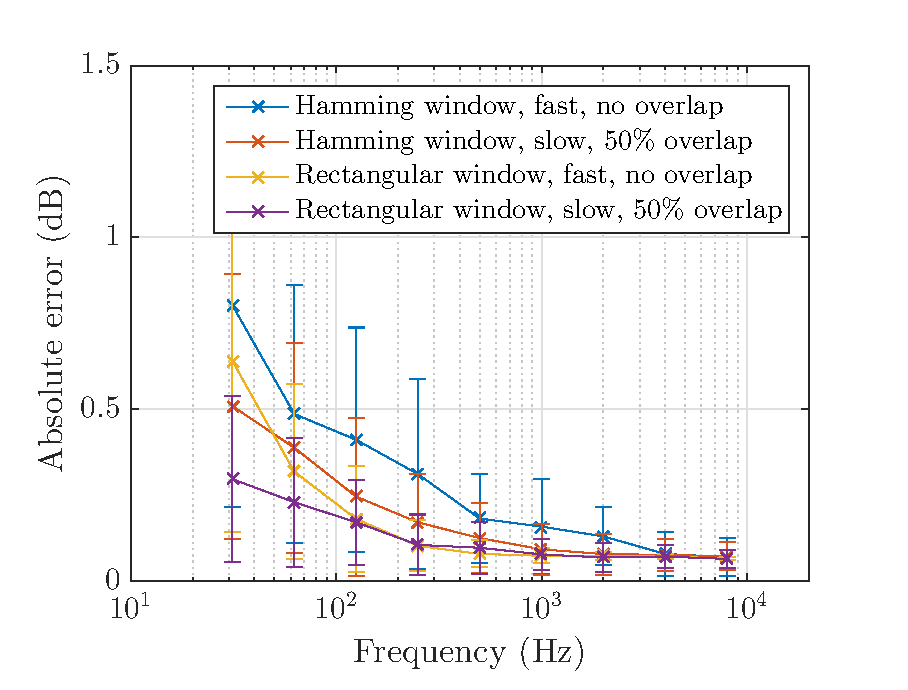
\includegraphics[width=\linewidth]{figures/err_m_n.eps} 
        \caption{Noise extracts}
    \end{subfigure}
    \hfill
    \begin{subfigure}[h]{0.45\textwidth}
        \centering
        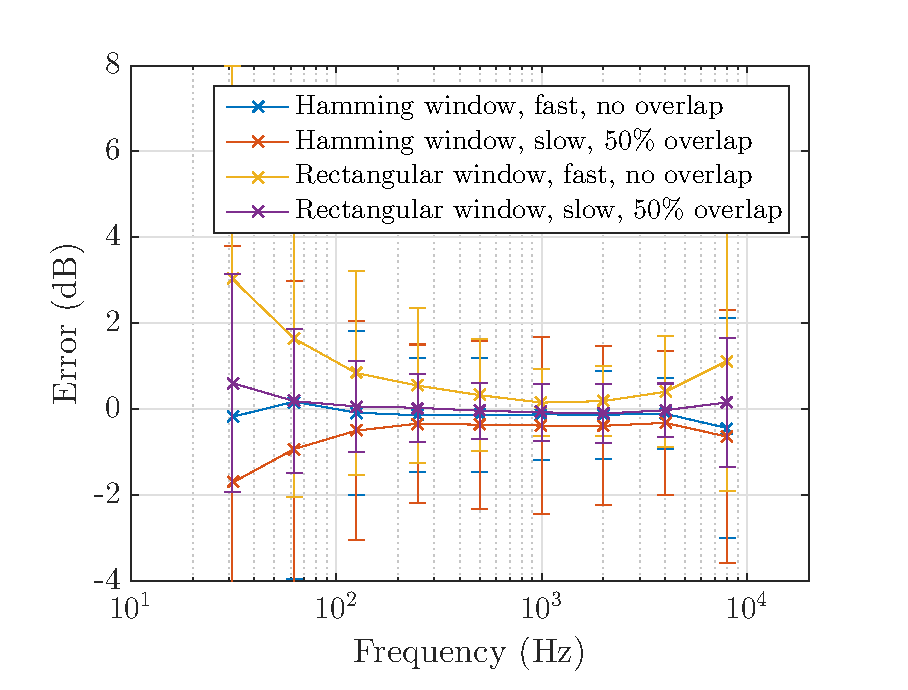
\includegraphics[width=\linewidth]{figures/err_m_u.eps} 
        \caption{Urban sounds recordings}
    \end{subfigure}
    \caption{\label{fig:error_m}Measurement error of third-octave bands over two-seconds recordings. The analysis of short frames has an effect on energy estimation at low frequencies. Framing is more impactful on signals where the energy is localized in frequency.}
\end{figure*}

To prove that the FFT-based method is not solely responsible for these errors, third-octave bands are computed via the \textit{ita\_toolbox} reference for the same parameters (fast and slow, windowing, overlap). It is found that for all parameters and all bands, except for the five lower frequency bands in fast analysis, the resulting errors are not statistically different to those obtained with the proposed method. For the remaining bands, the toolbox shows slightly higher or lower errors.

\paragraph{Encoding error\\\\}
The additional error caused by the encoding steps after obtaining the desired data representation, with the word size $q$ varying. Figure~\ref{fig:error_q} shows an estimation of the error $\hat{\varepsilon}$ as a function of $q$ for third-octave and Mel bands. In both cases, the mean and standard deviation seem to decrease by a factor of 2 as $q$ increases. This is in accordance with the approximate theoretical expressions obtained in equation~\ref{eq:13}. This error is to be added to the measurement error discussed in the precedent section.

\begin{figure}[htbp]
	\centering
		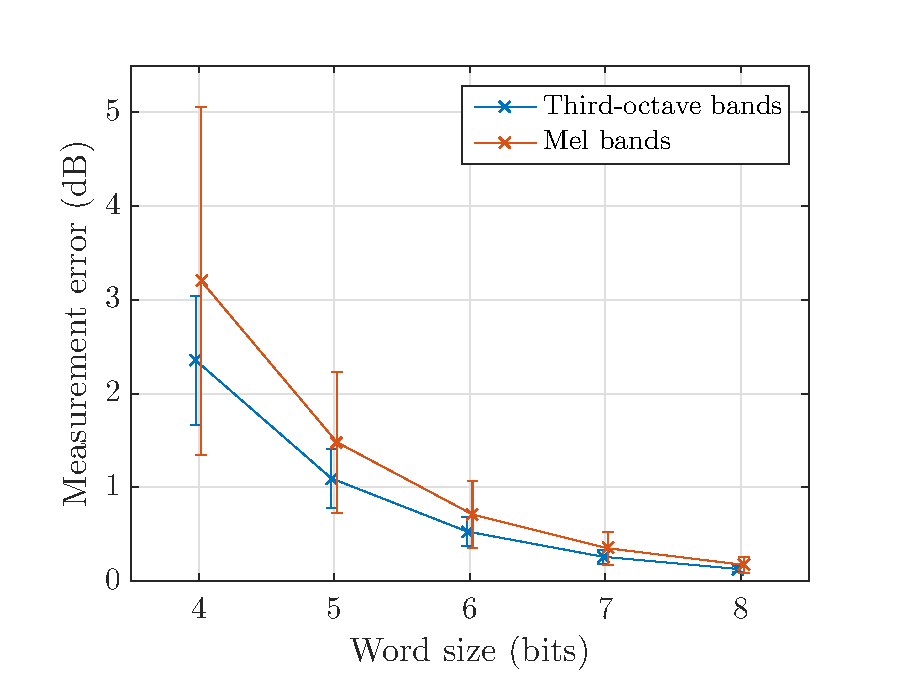
\includegraphics[width=0.7\columnwidth]{figures/error_qall.eps}
	\caption{Measurement error induced by encoding for different quantization resolutions.}
	\label{fig:error_q}
\end{figure}

\subsection{Output bitrate}
The main indicator of performance is the bitrate obtained at the output of the coder. The three varying factors studied are the data word size $q$, the number of bands and the effect of reducing time-resolution by averaging analysis frames. Figure~\ref{fig:bitrate_q} shows estimations of the output bitrate for different values of $q$. To match third-octave bands computation principle where a 125~ms analysis is mandatory, Mel frames were averaged over time. Because we use the most common parameters, namely 23.2~ms window with 50\% overlap, the closest achievable rate considering simple averaging is 7.74 frames per second. Third-octave representation on 31 bands yielded an overall higher size than their Mel equivalent, here estimated for 30 bands. It however compares with the 40-Mel bands representation which is the most used features in literature. This higher bitrate is likely due to the distribution observed by the data prior to Huffman encoding.\\

\begin{figure}[htbp]
	\centering
		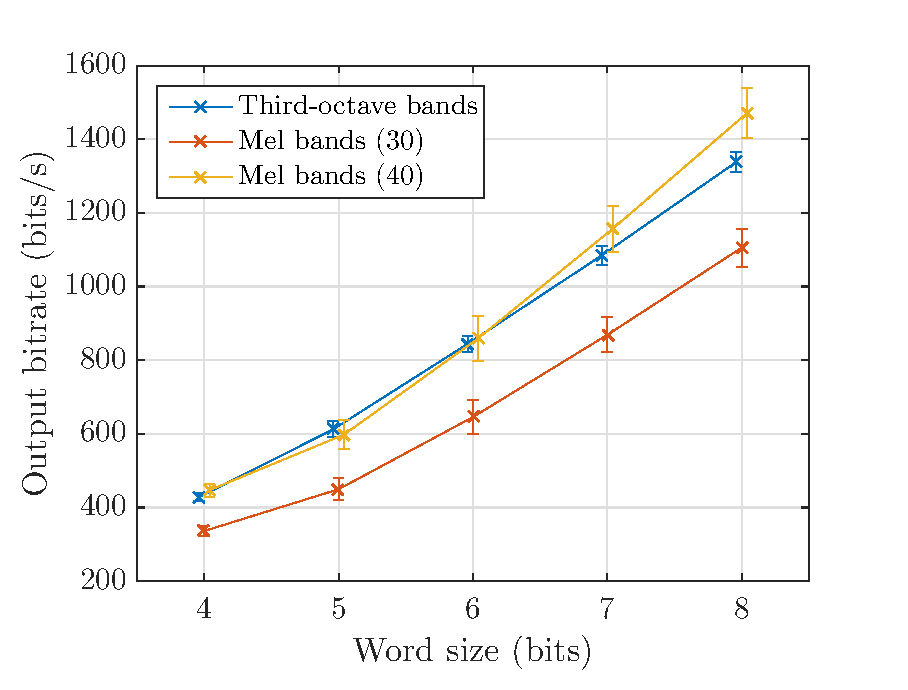
\includegraphics[width=0.7\columnwidth]{figures/bitrate_qall.eps}
	\caption{Coder output bitrate as a function of quantization for third-octave and Mel bands with 8 frames per second.}
	\label{fig:bitrate_q}
\end{figure}

A second set of parameters influences directly the time-frequency resolution of the analysis. By choosing a frame rate and number of bands, one can effectively control the size of periodically transmitted data. The bitrate is evaluated for 10 to 40 Mel bands and a frame rate from 2 to 10 per second, with fixed $q = 8$. Results are shown in Figure~\ref{fig:bitrate_mel_avg}. As expected, the bitrate for a given word size $q$ can be modeled as a linear function of the representation dimensions for one second of analysis. Small variations are induced by data distributions on a per-frame level and their impact on the Huffman algorithm.\\

\begin{figure}[htbp]
	\centering
		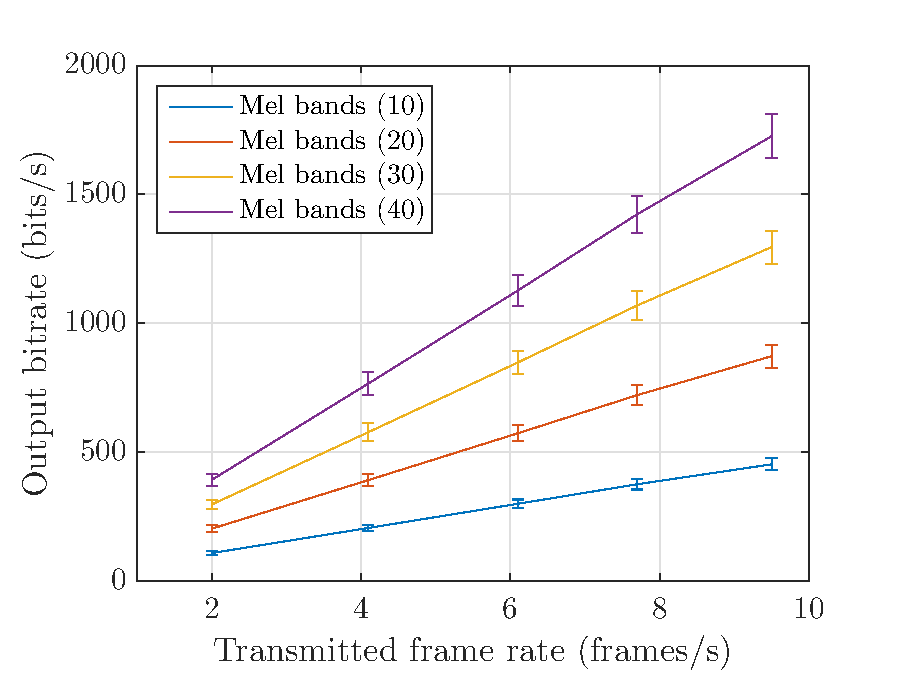
\includegraphics[width=0.7\columnwidth]{figures/bitrate_mel_avg.eps}
	\caption{Impact of representation resolution on the encoded data bitrate.}
	\label{fig:bitrate_mel_avg}
\end{figure}


\subsection{Event recognition}

The same set of parameters as in bitrate evaluation is used to study the impact of their tuning to the sound event recognition performance. The experiment is aimed at finding ways to further reduce the encoded data size without strongly affecting recognition performance. Results of the four presented classification methods are provided for the sake of completeness.\\

First, the impact of quantization on classification accuracy can be observed. The models are trained on the most complete implemented representation, ie. 40 Mel bands, 23.2~ms, 50\% overlap and no time averaging (85 frames per second). Figure~\ref{fig:class_mel_q} shows that this process yields equivalent accuracy for higher resolutions.\\

\begin{figure}[htbp]
	\centering
		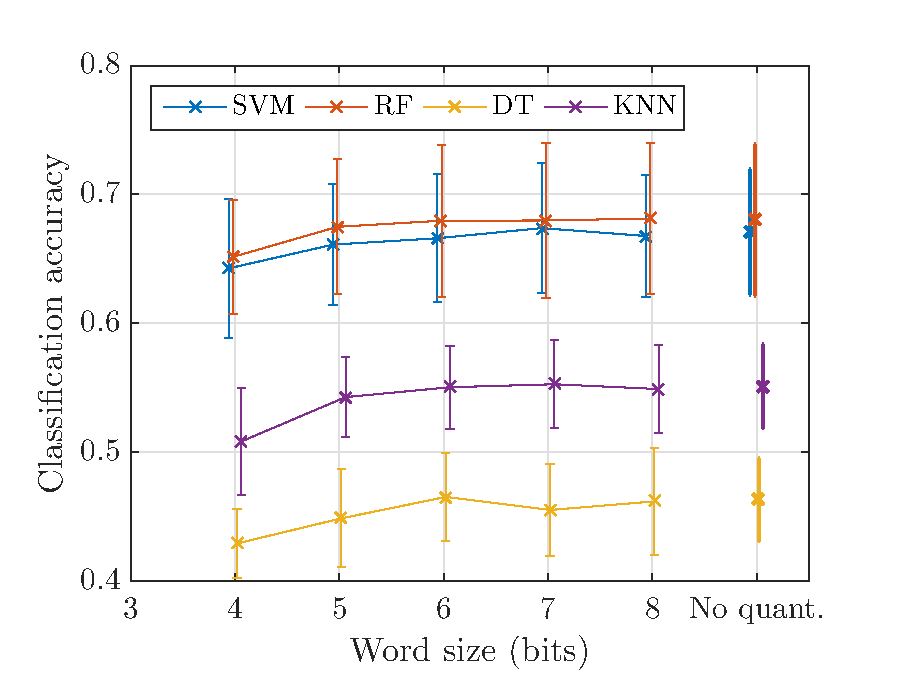
\includegraphics[width=0.7\columnwidth]{figures/class_mel_q.eps}
	\caption{Classification accuracy as a function of word size before encoding. The baseline on the right is computed without quantizing the representation.}
	\label{fig:class_mel_q}
\end{figure}

The effect of changing the time-frequency resolution of the representation is presented in Table~\ref{T2}. Similarly to baseline results, the random forest and SVM classifiers are the higher performing systems at $0.69\pm 0.06$ and $0.68\pm 0.04$ respectively. However, it is found that given our setup, reducing the number of analysis bands up to a given level most often does not induce a strong drop of performance. The performance of the decision tree classifier is a good example of this behavior, with best performances for 10 Mel bands only and a 4\% lower accuracy for 40. The latter result may be due to the low ability of the decision tree classifier to handle hugh dimensional features. Even if the difference is small, all other models perform best with 30 or 40 Mel bands as a representation. Time decimation cn also be considered, as the original representation can be averaged and consistently yield a good classification accuracy. The loss of information can be considered negligible for FPS values as low as 20 or 10 depending on the method. Even below, classification accuracy only drops by one or a few percents. This means that the data size can be effectively divided by a factor of at most 10 without strongly affecting sound event recognition performance. It also provides us with a preliminary confirmation of the possibility for "fast"-sampled third-octave bands cepstra to match MFCC performances.\\

\begin{table*}[h!]
\centering
\caption{Classification accuracy in percentage for different classifiers: SVMs (a), Random Forests (b), Decision Trees (c), and Nearest Neigbors (d) with respect to varying representation resolutions. Numbers in red indicate best performance and numbers in bold indicate statistical equivalent results compared to the best performing setting.}
\label{T2}
(a)\\
\begin{tabular}{ll|c|c|c|c|c|c|c|}
\cline{3-9}
\multicolumn{2}{c}{\multirow{2}{*}{SVM}} & \multicolumn{7}{|c|}{Frames per second}\\ \cline{3-9}
 & & 2 & 4 (4.1) & 6 (6.1) & 8 (7.7) & 10 (9.5) & 20 (21) & 85 \\ \cline{1-9}
\multicolumn{1}{|c}{\multirow{4}{*}{Mel bands}}
 & \multicolumn{1}{|c|}{10} & 55$\pm$3 & 60$\pm$3 & 61$\pm$4 & 62$\pm$3 & 62$\pm$4 & \textbf{63$\pm$6} & \textbf{65$\pm$6} \\ \cline{2-9}
\multicolumn{1}{|c}{}
 & \multicolumn{1}{|c|}{20} & 58$\pm$4 & 62$\pm$4 & 63$\pm$4 & 64$\pm$4 & 63$\pm$4 & \textbf{65$\pm$5} & \textbf{67$\pm$6} \\ \cline{2-9}
\multicolumn{1}{|c}{}
 & \multicolumn{1}{|c|}{30} & 60$\pm$3 & 64$\pm$4 & 64$\pm$4 & \textbf{65$\pm$4} & \textbf{65$\pm$3} & \textbf{67$\pm$4} & \textbf{\textcolor{red}{68$\pm$4}} \\ \cline{2-9}
\multicolumn{1}{|c}{}
 & \multicolumn{1}{|c|}{40} & 60$\pm$3 & 63$\pm$4 & \textbf{64$\pm$4} & 64$\pm$4 & \textbf{64$\pm$4} & \textbf{66$\pm$4} & \textbf{68$\pm$5} \\ \cline{1-9}
\end{tabular}
\\(b)\\
\begin{tabular}{ll|c|c|c|c|c|c|c|}
\cline{3-9}
\multicolumn{2}{c}{\multirow{2}{*}{RF-500}} & \multicolumn{7}{|c|}{Frames per second}\\ \cline{3-9}
 & & 2 & 4 (4.1) & 6 (6.1) & 8 (7.7) & 10 (9.5) & 20 (21) & 85 \\ \cline{1-9}
\multicolumn{1}{|c}{\multirow{4}{*}{Mel bands}}
 & \multicolumn{1}{|c|}{10} & 60$\pm$3 & 62$\pm$3 & 62$\pm$3 & 63$\pm$3 & 63$\pm$3 & \textbf{65$\pm$4} & \textbf{67$\pm$5} \\ \cline{2-9}
\multicolumn{1}{|c}{}
 & \multicolumn{1}{|c|}{20} & 61$\pm$4 & 63$\pm$3 & 64$\pm$3 & 64$\pm$3 & 64$\pm$4 & \textbf{66$\pm$6} & \textbf{69$\pm$6} \\ \cline{2-9}
\multicolumn{1}{|c}{}
 & \multicolumn{1}{|c|}{30} & 62$\pm$3 & 63$\pm$3 & 64$\pm$3 & 64$\pm$3 & 64$\pm$4 & \textbf{67$\pm$5} & \textbf{\textcolor{red}{69$\pm$6}} \\ \cline{2-9}
\multicolumn{1}{|c}{}
 & \multicolumn{1}{|c|}{40} & 62$\pm$4 & 63$\pm$4 & 63$\pm$4 & 64$\pm$4 & 63$\pm$4 & \textbf{67$\pm$6} & \textbf{68$\pm$6} \\ \cline{1-9}
\end{tabular}
\\(c)\\
\begin{tabular}{ll|c|c|c|c|c|c|c|}
\cline{3-9}
\multicolumn{2}{c}{\multirow{2}{*}{DT}} & \multicolumn{7}{|c|}{Frames per second}\\ \cline{3-9}
 & & 2 & 4 (4.1) & 6 (6.1) & 8 (7.7) & 10 (9.5) & 20 (21) & 85 \\ \cline{1-9}
\multicolumn{1}{|c}{\multirow{4}{*}{Mel bands}}
 & \multicolumn{1}{|c|}{10} & 42$\pm$3 & \textbf{46$\pm$4} & 46$\pm$2 & 44$\pm$3 & 45$\pm$3 & \textbf{46$\pm$5} & \textbf{\textcolor{red}{49$\pm$3}} \\ \cline{2-9}
\multicolumn{1}{|c}{}
 & \multicolumn{1}{|c|}{20} & 43$\pm$5 & 43$\pm$3 & 43$\pm$2 & 44$\pm$3 & 45$\pm$3 & 45$\pm$5 & \textbf{47$\pm$5} \\ \cline{2-9}
\multicolumn{1}{|c}{}
 & \multicolumn{1}{|c|}{30} & 42$\pm$4 & 43$\pm$2 & 44$\pm$3 & 45$\pm$5 & 43$\pm$3 & 43$\pm$4 & \textbf{45$\pm$5} \\ \cline{2-9}
\multicolumn{1}{|c}{}
 & \multicolumn{1}{|c|}{40} & 42$\pm$6 & 43$\pm$3 & 43$\pm$3 & 42$\pm$3 & 44$\pm$3 & 46$\pm$3 & \textbf{46$\pm$4} \\ \cline{1-9}
\end{tabular}
\\(d)\\
\begin{tabular}{ll|c|c|c|c|c|c|c|}
\cline{3-9}
\multicolumn{2}{c}{\multirow{2}{*}{KNN-5}} & \multicolumn{7}{|c|}{Frames per second}\\ \cline{3-9}
 & & 2 & 4 (4.1) & 6 (6.1) & 8 (7.7) & 10 (9.5) & 20 (21) & 85 \\ \cline{1-9}
\multicolumn{1}{|c}{\multirow{4}{*}{Mel bands}}
 & \multicolumn{1}{|c|}{10} &43$\pm$2 & 51$\pm$4 & 53$\pm$4 & 53$\pm$5 & 53$\pm$4 & 54$\pm$4 & \textbf{56$\pm$3} \\ \cline{2-9}
\multicolumn{1}{|c}{}
 & \multicolumn{1}{|c|}{20} & 44$\pm$3 & 52$\pm$4 & 53$\pm$3 & 54$\pm$4 & \textbf{54$\pm$4} & \textbf{55$\pm$4} & \textbf{\textcolor{red}{58$\pm$4}} \\ \cline{2-9}
\multicolumn{1}{|c}{}
 & \multicolumn{1}{|c|}{30} & 45$\pm$4 & 54$\pm$5 & \textbf{55$\pm$5} & \textbf{55$\pm$4} & \textbf{55$\pm$4} & \textbf{56$\pm$4} & \textbf{56$\pm$4} \\ \cline{2-9}
\multicolumn{1}{|c}{}
 & \multicolumn{1}{|c|}{40} & 46$\pm$3 & 53$\pm$5 & \textbf{55$\pm$5} & \textbf{55$\pm$4} & \textbf{55$\pm$5} & \textbf{57$\pm$4} & \textbf{57$\pm$3} \\ \cline{1-9}
\end{tabular}

\end{table*}

The next test compares the efficiency of third-octave bands at characterizing urban soundscapes to that of Mel spectrograms. Following the previous discussions, the classification task is run on corresponding cepstra with a fixed 8 frames per second and 31 bands. Figure~\ref{fig:class_tob_q} displays similar results to the 40 bands, 8 fps Mel spectrograms seen in Table~\ref{T2} for all classification schemes. In this table, equivalence of performance with respect to the best performing setting (in red) is depicted with a bold font evaluated using the following procedure. The null hypothesis that the subtraction of the two compared distribution (the distribution of the consider setting minus the distribution of the best performing one) comes from a normal distribution with mean equal to zero and unknown variance is evaluated using the paired-sample t-test at the 0.05 significance level. If the null hypothesis is not rejected, the setting is considered as equivalent in terms of performance to the best performing one.\\

\begin{figure}[htbp]
	\centering
		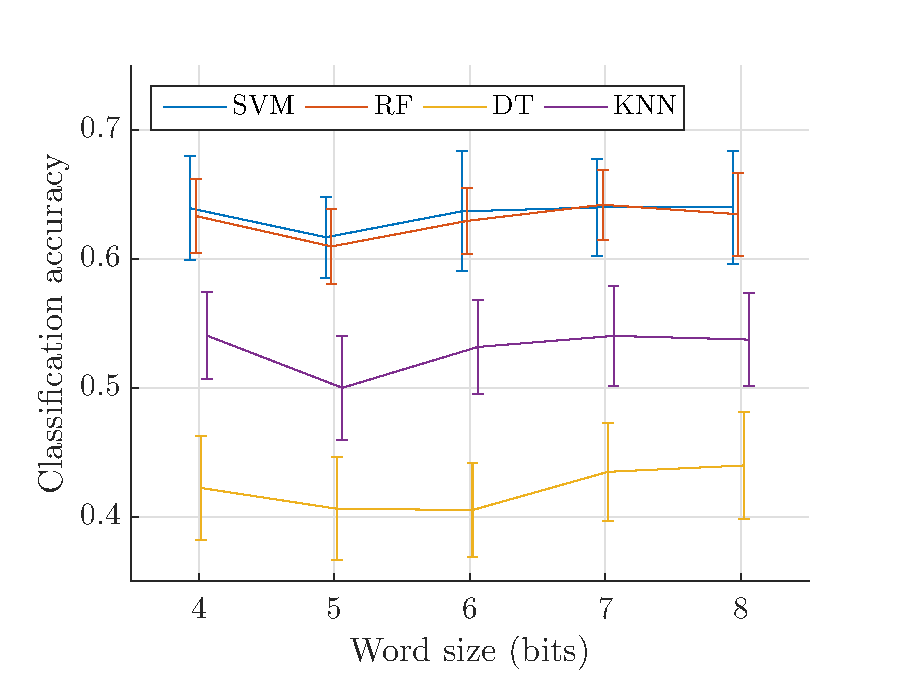
\includegraphics[width=0.7\columnwidth]{figures/class_tob_q.eps}
	\caption{Classification accuracy with third-octave bands and varying word size.}
	\label{fig:class_tob_q}
\end{figure}

To further analyze both representations advantages, the confusion matrix is a reliable tool. It aims at providing information regarding class-by-class accuracy and misclassification rates. Confusion matrices are thus computed for the SVM classifier, with predictions accumulated over the ten folds in test configuration. The analogous natures of the two descriptors is highlighted by close one-versus-one differentiation performances, with a slightly lower accuracy for third-octave bands on average. Both representations yield best results for the \textit{Gun shot} class with 88.2\% for third-octave cepstra and 86.6\% for Mel cepstra. Their poorest accuracy is on the \textit{Air conditioning} class with 32.0\% and 38.1\% respectively. However, a noticeable difference between them is that on the log-frequency scale the bandwidth of Mel filters narrows as frequency increases, while third-octave are evenly distributed. The effect of this can be seen between classes \textit{Drilling} and \textit{Jackhammer}. These sounds involve important low-frequency information which can generally differentiate them, leading third-octave descriptors to perform better. Conversely, using Mel-based cepstra improves globally \textit{Air conditioning} recognition as most of its defining components are situated in higher frequencies.\\

Both descriptor are thus found to have similar representational capabilities despite minor differences due to their respective designs.

\subsection{Intelligibility}

Objective intelligibility metrics are then computed for the encoder's settings under evaluation and compared to the results of the perceptual test. The results of the perceptual test is evaluated using the average intelligibility score (AIS) given by the subjects and the intelligibility ratio (IR) computed as the number of correctly transcribed words versus the number of words in the spoken utterance. Figure~\ref{fig:subj_int} presents the results of the perceptual test for the same encoder's settings, Figure~\ref{fig:csii_tob_fps} and Figure~\ref{fig:fwsnrseg_tob_fps} show the CSII and fwSNRseg estimations respectively.

Perceptual test results confirm the qualitative evaluation of speech properties discussed in Section \ref{sec:unintelligibility}. Phonemes separation is indeed mandatory in order to ensure good intelligibility of speech. This implies an analysis frame rate significantly larger than the phonemes rate the considered language. A limit of about 10~Hz corresponding to a frame duration of 100~ms is observed, as the studied 8~Hz setting is found to be almost completely unintelligible. Very few words are understood correctly. It can be assumed that correctly identified words are a result of coincidentally adequate frame timings, \textit{i.e.} analysis frames matching the location of phoneme utterances for a short duration. Similarly, framing effects induced by the proposed processing scheme yielded errors for higher frame rates transcriptions and a globally lower perceptual intelligibility.\\


\begin{figure}[htbp]
	\centering
		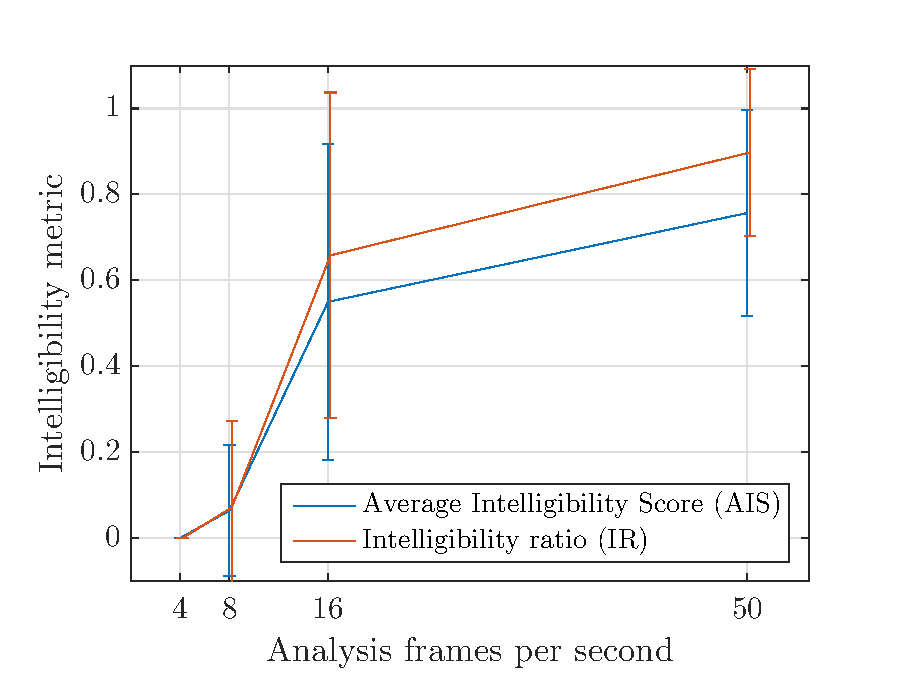
\includegraphics[width=0.7\columnwidth]{figures/subj_int.eps}
	\caption{Average intellibility score (AIS) given by the subjects and the inteligibility ratio (IR) as a function of the frame rate. Unintelligibility appears at around 10~Hz, corresponding to the average duration of a phoneme.}
	\label{fig:subj_int}
\end{figure}

The CSII accounts for the distance between clean and distorted audio spectrograms at each point in time and frequency. This includes the phase, which we discard early in the representation step. The error induced by forward and inverse third-octave bands transformation as well as operations reducing data bitrate further contribute to very high element-wise disparities. In fact, the signal is too distorted for the proposed SNR normalization to ensure CSII values in the 0-1 range. When compared to perceptual test results, the CSII shows no clear separation in the 10 frames per second neighbourhood. It is therefore not a good indicator in the studied conditions.\\

\begin{figure}[htbp]
	\centering
		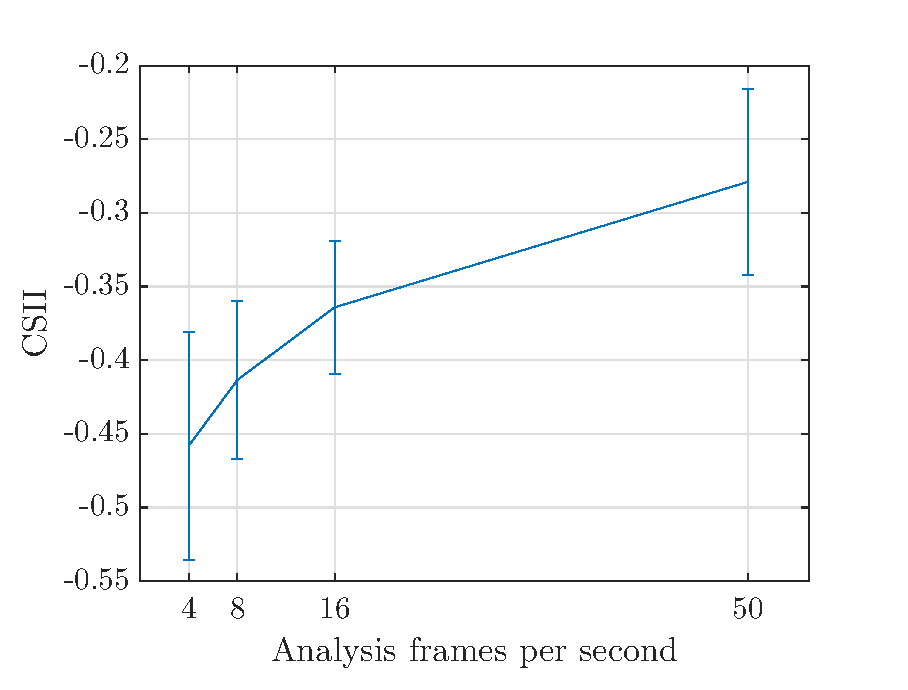
\includegraphics[width=0.7\columnwidth]{figures/csii_tob_fps.eps}
	\caption{The Coherence SII objective indicator computed for intelligibility assessment. Negative CSII values indicate a signal-to-noise ratio too low for the recommended normalization, thus severe disparities between the original and reconstructed signal.}
	\label{fig:csii_tob_fps}
\end{figure}

Alternatively, the frequency-weighted segmental SNR considers only spectrogram magnitudes. As a result, distance is generally lower and more representative of the induced perceptual distortion. Nevertheless, the fwSNRseg still uses a point-wise comparison which is certainly too precise for the studied degradations. Its shape seems more accurate at higher frame rates where intelligibility is almost constant. The previously observed threshold is however absent as the curve present a smoother increase trend, and the difference between 8~Hz and 16~Hz is not significant enough to correlate with subjective measurements.\\

\begin{figure}[htbp]
	\centering
		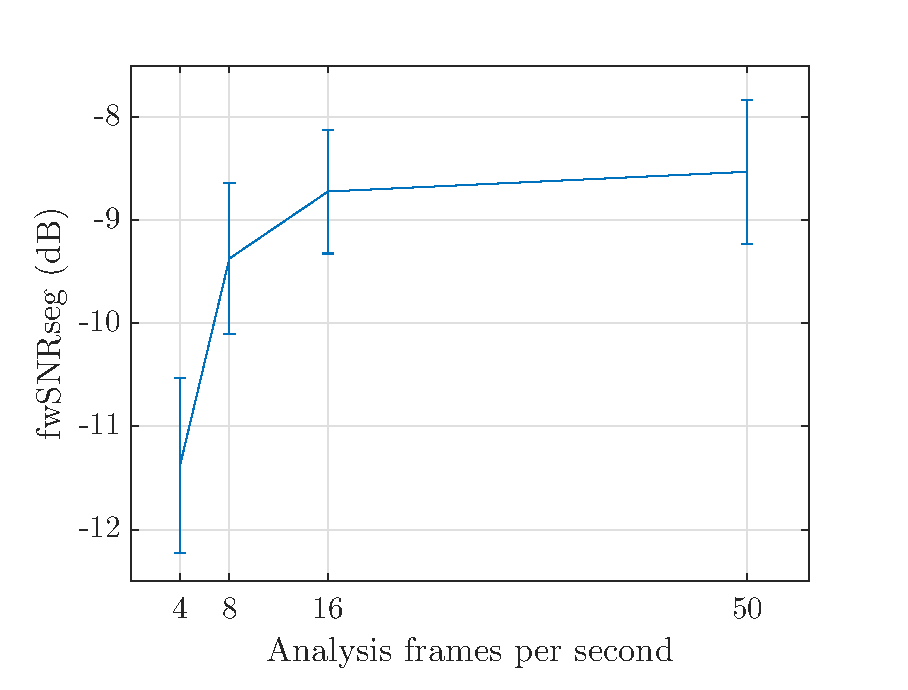
\includegraphics[width=0.7\columnwidth]{figures/fwsnrseg_tob_fps.eps}
	\caption{Frequency-weighted segmental SNR with varying analysis frame rates around the considered 8~Hz value. This indicator shows a better correlation with subjective tests but lacks an inintelligibility threshold.}
	\label{fig:fwsnrseg_tob_fps}
\end{figure}

\clearpage
\part{Personal report}

This part provides personal views and perspectives regarding this internship, both retrospectively and about its implication on my future development. To this aim, the recurring technical and human challenges, opportunities and discoveries will be detailed.\\

The main technical issue encountered still follows my work. I had indeed poor initial knowledge on acoustics and only basic audio signal processing. Either to correctly design the system or to interpret results, I often had to read entire book chapters about new notions. Fortunately, my referent professor and other people I interacted with were always willing to help by providing me with either written material, oral explanations or even a course. I continue to view this concern as an opportunity to enrich the yet small extent of my knowledge.\\

A second major technical problem was the computation of third-octave bands measurement error. The issue had multiple factors. First, I did not have access to the full text of standards about this indicator and thus only had approximate tolerances to work with. Second, there was a lack of reference implementation to compare with. The ita\_toolbox supposedly was one, but that was never really demonstrated in the studied conditions of short-time analysis. Third, there was also a lack of clear experimental setup. The error was computed as an absolute difference, which is only sensible if the unit of measurements is disregarded. Uncertainties on the nature of the quantities to compare were also regularly discussed. A significant amount of time was spent in trying to solve this problem with acousticians at IFSTTAR, that while important was subsidiary to the internship's objective.\\

Organization-wise, I often misjudged the duration of certain tasks leading to previsional plannings not being fully met. Similarly, some of my priorities were suboptimal and I had difficulties stopping on more delicate, less secondary problems. Every mistake is however an opportunity to learn and I retrospectively do not view these issues as failures.\\

Working alone on a daily basis, though evidently expected in an academic environment, was arduous at times. However, this issue did not have as important an impact as I first imagined. In fact, apart from a few moments towards three months after the beginning of the internship, I quickly started adapting to this concept and it never really slowed my progress. In this respect, this six month long working experience was formative. It introduced me to a different method as opposed to the teamwork-oriented approach I was familiar with, effectively adjusting my organization as it can be expected as part of a PhD thesis preparation.\\

Overall this masters internship was an accurate preview of the academic and research world in which I intend to develop. I was familiarized with the specific technical knowledge on experimental rules, results interpretation, paper writing and bibliographical search among others. New work organization elements were also addressed, as well as project management tools and practices. Lastly, I was introduced to a passionate and open community which corresponds in every respect to my expectations.\\


\clearpage
\section*{Conclusion}
\addcontentsline{toc}{section}{Conclusion}
This report presented the work accomplished during this six-months masters internship. An audio coder scheme has been developed which allows the computation of acoustic indicators and sound event recognition while degrading the intelligibility of speech. It also fullfills the requested constraints in terms of bitrate and computational complexity.\\


This internship was rich in multiple aspects. My working activity involved diverse domains of technical skills, previously unknown for some, and tested a significant part of my training. The CENSE project is the first truly large project that I am a part of, with more than ten member entities with strong expertise in their own domain working together towards solving a single problem. My exchanges with researchers and engineers in other areas allowed me to understand the views, aims and concerns of each and provided me with an accurate insight about large research projects.\\

I also acquired a global vision on the research and academic environment. This includes time and resources management, project development, technical practices and several other points ranging from information on scientific journals organization to complete experiment management methods.\\

The internship comforted me in my decision to pursue a PhD thesis. I look forward to the three upcomung years during which part of my work will benefit the CENSE project. This will also allow me to follow the implications of the scheme I helped develop for its embedded implementation and operation. A journal paper will be submitted to a special issue on smart cities of the MDPI Sensors journal (impact factor 2.6) in the next few months.

\clearpage
\appendix
\section{Signal reconstruction techniques}
\label{sigrec}
While reversing the data encoding step is straightforward, reconstructing audio from a frequency band representation is not trivial. The forward transform discards part of the information that the original recording contained: first when omitting spectrogram phase data, then when applying the linear transform that defines band analysis.
\subsection{Spectrogram computation from band representations}
The operation applied to obtain a band representation $T$ from a linearly-scaled spectrogram $X$ of size $m\times n$ can in the general case be written as:
\begin{equation}
T = MX
\end{equation}
with $M$ the transform matrix of size $k\times m, k<m$. The operation is thus essentially an averaging, and by definition there exist no single solution $N$ such as $NT = X$, that is $NM = I_m$. The matrix used to recover the linearly-scaled spectrogram must therefore be estimated. This is possible by scaling the transpose of $M$:
\begin{equation}
\hat{N} = \frac{1}{a}M^T
\end{equation}
where $a$ is a normalization scalar usually expressed as $a = c\cdot diag(M^TM)$ with $c$ a numerical constant.\\

This estimation does not yield a perfect reconstruction of the spectrogram, as can be seen in Figure~\ref{fig:freq}. The resulting effect can be interpreted as a heterogeneous loss of resolution that increases with frequency bands. Each frequency bin of the linear spectrogram is averaged with other bins that belong to the same band.

\begin{figure}[htbp]
	\centering
		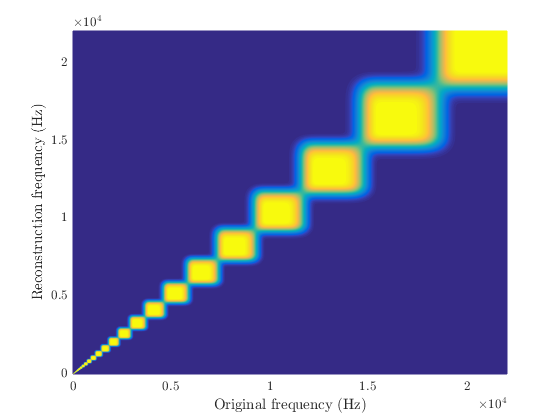
\includegraphics[width=0.7\columnwidth]{figures/freq.png}
	\caption{Third-octave bands analysis and approximate inverse transformation effects on energy location. This process yields an important and heterogeneous loss in resolution, particularly at higher frequency points.}
	\label{fig:freq}
\end{figure}

\subsection{Phase recovery}
A large number of methods exist to reconstruct the phase from spectrogram magnitude. An extensive review of such methods is available in \cite{sturmel2011}. In the scope of this application, the Griffin and Lim algorithm \cite{griffin1984} is used. It consists in computing successive estimations $\tilde{x}$ of the signal $x$ by repeating the process:
\begin{align}
\tilde{X}_{i}(k, f) &= STFT(\tilde{x}_{i}[n])\\
\tilde{X}_{i+1}(k, f) &= |X(k, f)|\frac{\tilde{X}_{i}(k, f)}{|\tilde{X}_{i}(k, f)|}\\
\tilde{x}_{i+1}[n] &= STFT^{-1}(\tilde{X}_{i+1}(k, f))
\end{align}
for a fixed number of iterations $i$ or until convergence. The estimate $\tilde{x}_0$ is usually initialized with random numbers or zeros.


\clearpage
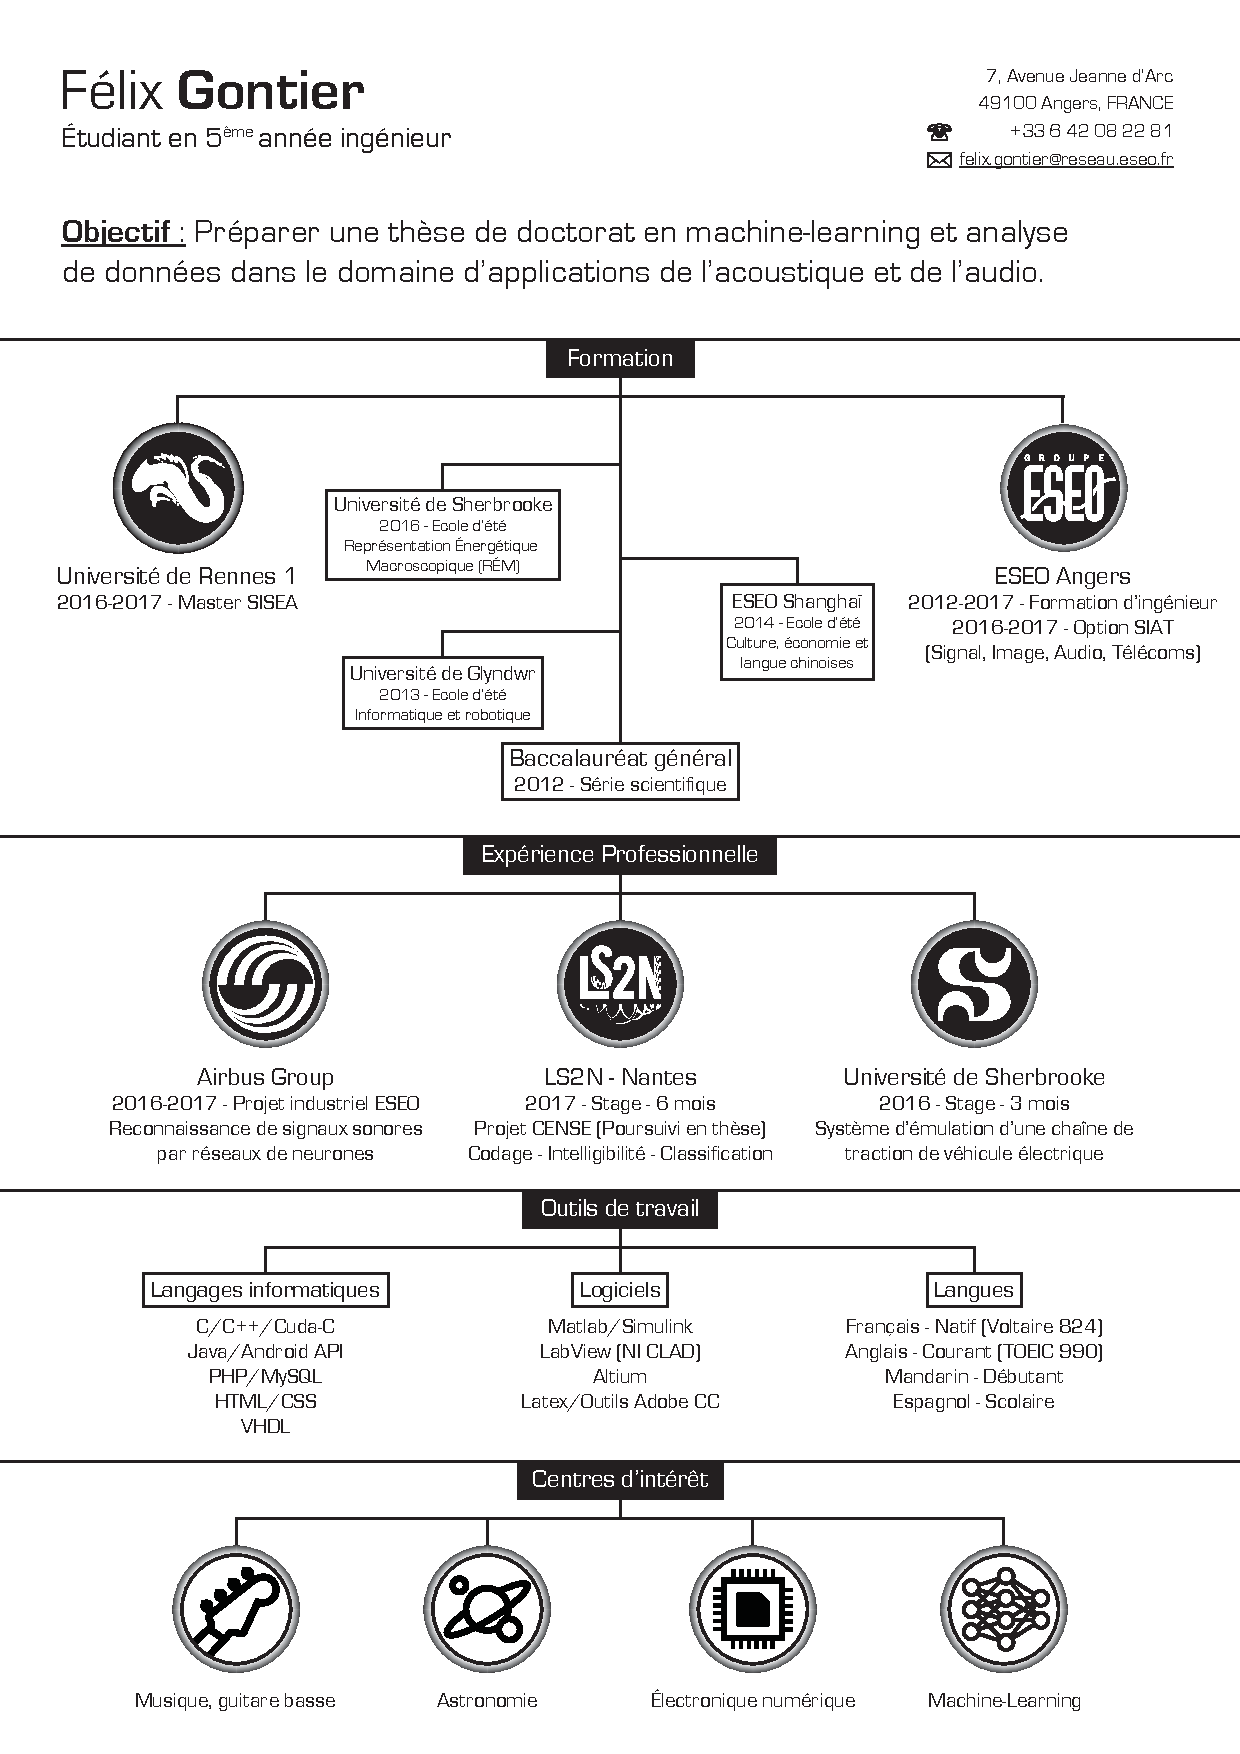
\includepdf[pages={1}]{cv.pdf}

\bibliographystyle{plain}
\bibliography{biblio}


\end{document}

\endinput
%%
%% End of file `elsarticle-template-harv.tex'.
